%%\documentclass[usenatbib,usegraphicx,letterpaper]{mnras}
\documentclass[usenatbib]{mnras}
%%\usepackage[totalwidth=480pt,totalheight=680pt]{geometry}
\usepackage{amssymb}
\usepackage{epsfig}
\usepackage{amsmath}
\usepackage{color}
\usepackage[dvipsnames]{xcolor}
\usepackage{epsfig}  
\usepackage{graphicx}
\usepackage{subfig}
\usepackage{rotating}
\usepackage{fixltx2e}
%%\usepackage{physics}

%Journals
\def\pasj{{PASJ}}
\def\nat{{ Nature }}
\def\aap{{ Astron. \& Astrophys. }}
\def\aj{{ Astron.~J. }}
\def\apj{{ Astrophys.~J. }}
\def\araa{{ Ann. Rev. Astron. Astrophys. }}
\def\apjl{{ Astrophys.~J.~Letters }}
\def\apjs{{ Astrophys.~J.~Suppl. }}
\def\apss{{ Astrophys.~Space~Sci. }}
\def\icarus{{ Icarus }}
\def\mnras{{ MNRAS }}
\def\pasp{{ Pub. Astron. Soc. Pacific }}
\def\planss{{ Plan. Space Sci. }}
\def\physrep{{ Phys. Rep.}}
\def\jcap{{J. Cosm. Astropart. Phys.}}

% less then similar, greater than similar
\def\lsim{\lower0.6ex\vbox{\hbox{$ \buildrel{\textstyle <}\over{\sim}\ $}}}
\def\gsim{\lower0.6ex\vbox{\hbox{$ \buildrel{\textstyle >}\over{\sim}\ $}}}

% begin equation
\newcommand{\beq}{\begin{equation}}
\newcommand{\eeq}{\end{equation}}
\newcommand{\beqa}{\begin{eqnarray}}
\newcommand{\eeqa}{\end{eqnarray}}

% basic cosmology
\newcommand{\Ho}{H_{0}}
\newcommand{\Om}{\Omega_{\mathrm{M}}}
\newcommand{\Ol}{\Omega_{\Lambda}}
\newcommand{\Ode}{\Omega_{\mathrm{DE}}}
\newcommand{\rhocrit}{\rho_{\mathrm{crit}}}
\newcommand{\Ok}{\Omega_{\mathrm{K}}}
\newcommand{\wzero}{w_{0}}
\newcommand{\wa}{w_{\mathrm{a}}}
\newcommand{\wpiv}{w_{\mathrm{piv}}}
\newcommand{\apiv}{a_{\mathrm{piv}}}
\newcommand{\ellmax}{\ell_{\mathrm{max}}}
\newcommand{\fsky}{f_{\mathrm{sky}}}

\newcommand{\fom}{\mathcal{F}}
\newcommand{\Rvir}{r_{\mathrm{vir}}}
\newcommand{\Rdel}{r_{\Delta}}

% units
\newcommand{\Msun}{\mathrm{M}_{\odot}~}
\newcommand{\hMsun}{\ h^{-1}\mathrm{M}_{\odot}~}
\newcommand{\hMpc}{\ h^{-1}\mathrm{Mpc}~}
\newcommand{\hkpc}{\ h^{-1}\mathrm{kpc}~}
\newcommand{\cpiv}{c_{\mathrm{piv}}}
\newcommand{\kmsmpc}{~\mathrm{km/s/Mpc}~}
\newcommand{\kms}{~\mathrm{km}~\mathrm{s}^{-1}}
\newcommand{\Mpc}{\mathrm{Mpc}}
\newcommand{\kpc}{\mathrm{kpc}}
\newcommand{\pc}{\mathrm{pc}}
\newcommand{\au}{\mathrm{AU}}
\newcommand{\gev}{\mathrm{GeV}}

% roman differential
%\newcommand{\dd}{\mathrm{d}}

% comments
\newcommand{\arz}[1]{{\color{BrickRed}\textbf{[ARZ: }\textbf{#1}]}}


%%\bibliographystyle{mn2e}
\bibliographystyle{mnras}

%%%%%%%%%%%%%%%%%%%%%%%%%%%%%%%%%%%%%%%%%%%%%%%%

\begin{document}


\title[The Immitigable Nature of Assembly Bias]{The Immitigable Nature of Assembly
Bias: the Impact of Halo Definition on Environmental Effects}
\author[A. Villarreal et al.]{
Antonio S. Villarreal,$^{1}$\thanks{E-mail: asv13@pitt.edu}
Andrew R. Zentner,$^{1}$\thanks{E-mail: zentner@pitt.edu}
Christopher W. Purcell,$^{2}$\thanks{E-mail: cwpurcell@mail.wvu.edu}
\newauthor
Andrew P. Hearin,$^{3}$\thanks{andrew.hearin@yale.edu}
and Frank C. van den Bosch$^{3}$\thanks{frank.vandenbosch@yale.edu} 
\\
$^{1}$Department of Physics and Astronomy \& Pittsburgh Particle Physics,\\ Astrophysics, and Cosmology Center (Pitt-PACC), \\
University of Pittsburgh, Pittsburgh, PA\\
$^{2}$Department of Physics and Astronomy, \\
West Virginia University, Morgantown, WV \\
$^{3}$Department of Astronomy, \\
Yale University, Hew Haven, CT}

\date{In preparation}

%%\pagerange{\pageref{firstpage}--\pageref{lastpage}} \pubyear{2015}

%% \label{firstpage}

\maketitle

\begin{abstract}
%% Abstract goes here
Recent work has shown the importance of environment to the properties of dark matter halos. This brings conflict
to standard implementations of the halo model and excursion set theory which assume that the properties of a
population within the halo is determined by the mass of the halo alone. We seek to find a definition of the size
of a halo that allows us to minimize the impact of assembly bias on halo model calculations. We analyze the
dependence on environment of our properties using the method of marked correlation functions for several
different halo definitions, utilizing the \citet{diemer_kravtsov15} simulations. We find that the strength of assembly
bias has a strong dependence on the measured halo mass, even after the removal of gross mass dependencies at fixed
halo mass. We note that differences in halo definition, sample selection, and properties of interest can greatly impact
the measurement of assembly bias, potentially explaining conflicting results in the literature. These results suggest that
halo assembly bias appears increasingly difficult to resolve using the definitions common in current halo finder techniques,
possibly pointing toward the necessity of methods such as utilizing the halo splashback radius.
\end{abstract}

\begin{keywords}
cosmology: dark matter -- cosmology: large-scale structure of Universe -- galaxies: formation --galaxies: halos -- methods: numerical
\end{keywords}

%% notes on citation style:
%% \citep{stuff01,stuff02,stuff03} produces (Stuff 2001; Stuff 2002; Stuff 2003)
%% \citet{stuff04} produces "Stuff (2004)" in the main body
%% \\* defines a break in a section title it appears?
%% \begin{enumerate} into \item allows you to do the (i), (ii), (iii) thing 


\arz{We should add Andrew Hearin and Frank van den Bosch. Look into formatting the title correctly. Once I'm happy with the quality of the writing, we'll also need to send this to Benedikt Diemer and Andrey Kravtsov and offer them authorship.}

%-----------------------
\section{Introduction}
\label{section:introduction}
%-----------------------

In the concordance cosmology, galaxies and clusters form within merging dark matter halos \citep{white_rees78,blumenthal_etal84, mo_etal10}. Numerical simulations have provided a solid understanding of the abundances, properties, and 
clustering of dark matter halos in the standard cosmological model. Accordingly, it is possible to compute the 
clustering statistics of galaxies given a model for the (probabilistic) relationship between galaxies and dark matter halos. 
Such halo occupation models have been used to interpret large-scale structure measurements and 
constrain models of galaxy evolution \citep{yang_etal03,tinker_etal05,zehavi_etal05b,porciani_norberg06,vdbosch_etal07,zheng_etal07,conroy_wechsler09,
yang_etal09b,zehavi_etal11,guo_etal11a,wake_etal11,yang_etal11a,yang_etal12,leauthaud_etal12,
rodriguezpuebla_etal12, behroozi_etal13b, moster_etal13, tinker_etal13,cacciato_etal13,more_etal13,guo_etal14,
zu_mandelbaum15b}.
To date, the vast majority of halo occupation models rely on a key assumption, namely that 
the probability of a halo hosting a certain number of galaxies of a particular type 
depends only upon halo mass. It is now well known that the clustering strength of halos depends upon 
properties such as halo formation time \citep{gao_etal05,harker_etal06, wechsler_etal06,gao_white07,croton_etal07,zentner07,dalal_etal08, li_etal08, lacerna_padilla11}, 
concentration \citep{wechsler_etal06,faltenbacher_white10, mao_etal15}, and other halo properties \citep{bett_etal06, hahn_etal07a, hahn_etal07b, faltenbacher_white10, vandaalen_etal12, fisher_faltenbacher16, sunayama_etal16, chavesmontero_etal16}\arz{NEED SOME ADDITIONAL CITATIONS HERE.}. 
If galaxy properties depend upon these halo properties, a phenomenon known as galaxy {\em assembly bias}, 
then standard halo occupation modeling will fail \citep{zentner_etal14} 
and more complex models \citep{gilmarin_etal11, hearin_etal16} are necessary.


In this work, we explore the possibility of simplifying halo occupation modeling, at least for some 
applications, by altering the definition of a halo. Traditional definitions of halo boundaries are 
not particularly well motivated, so it seems natural to explore alternative definitions of halo size. 
Halo definitions have become a matter of convention that vary considerably in the literature. Many 
authors define halos using a friends-of-friend (FoF) algorithm applied to the particle distribution that designates 
halo boundaries as regions of roughly constant density. More often, authors define halos by spherical 
overdensity (SO) regions within which the mean density exceeds a particular threshold. The threshold used 
varies significantly. One difference is that some studies define the density threshold with respect to the 
mean background density, while others define the density threshold with respect to the critical density of 
the universe. Even when the same reference density is used, the threshold level varies. With respect to the 
mean density of the universe, commonly used thresholds are 178, 180, 200, and $\sim$340 times the mean 
background density, the last of these being the ``virial" overdensity in a concordance $\Lambda$CDM universe. 
Significantly higher values of the overdensity parameter are often used in studies of X-ray emission from cluster-sized halos. 
These definitions exclude particles that are gravitationally bound to the halo \citep{kazantzidis_etal06, valluri_etal07, more_etal15}. 


In this paper we explore the possibility of using halo definition to work for the 
convenience of the practitioner. We study the strength of various halo assembly bias signals 
as a function of halo definition. This is motivated, in large part, by recent literature that suggests 
that a large portion of the assembly bias signals are driven by halos in the relatively dense environments 
surrounding larger halos \citep{wang_etal07, warnick_etal08, more_etal15} and the fact
that the envionmental impact of halos has been shown to extend beyond well beyond the virial radius. \citep{adhikari_etal14, diemer_kravtsov14, wetzel_etal14, more_etal15, wetzel_nagai15} 
\arz{Need citations here to work by Wang (2007), the recent work on splashback (backsplash) 
and flyby halos, and the recent work on the splashback radius.} 
These halos have anomalous properties (e.g., formation times, concentrations, etc.) compared to field halos 
in part because of their interactions with their larger, neighbor halos. It seems interesting to ask whether or 
not defining halos to contain many of these anomalous neighbor halos, thus using the halo concept to draw a 
more meaningful boundary around regions within which highly nonlinear effects are important, can mitigate 
halo assembly bias. This is the aim of our paper. 


In the present paper, we restrict ourselves to halos that are defined by spherical regions and we 
study the strength of halo assembly bias as a function of the density threshold used to delineate these 
spherical halos. We find that for the properties tracing halo concentration, there exist scales and mass selections in which
assembly bias is mitigated for certain definitions of halo size. In particular, we note that the highest mass halos appear to have
minimal assembly bias at the fiducial halo definition, while low mass halos require a dramatic increase in halo size to accomodate for the
effect of assembly bias. We also find that this result does not hold for parameters such as halo shape, halo spin, or halo satellite number. 
We suggest that this result is consistent with current models of halo formation and suggests the impact of large scale structure on these 
parameters.\arz{two or three sentence, relatively non-technical summary of our results should go here.}

 
In \S~\ref{section:data} of this paper, we discuss the cosmological simulations that we analyze and how halos are
identified. In \S~\ref{section:haloprops}, we consider the properties of interest within our halo simulation and
their standard definitions. In \S~\ref{section:methodology}, we discuss the statistics that we use to measureeducing environmental effects through a
redefinition of halo environments and discuss possible applications of our methodology.
assembly bias and the removal of known mass scaling from our halo properties. In \S~\ref{section:results}, we
present our results and consider how the change of halo definition impacts measures of assembly bias. In
\S~\ref{section:conclusions}, we discuss the significance of r We also consider the
nature of assembly bias as a function of halo definition.





%------------------------------------
\section[]{Simulations and Halo Identification}
\label{section:data}
%------------------------------------

In order to study the effects of halo redefinition, we use three cosmological $N$-body simulations of structure
formation. The \citet{diemer_kravtsov15} simulations each utilize a Planck best-fit cosmology with $\Om = 0.32$, $\Ol =
0.68$, and $h_{\mathrm{o}} = 0.67$. We use three simulation boxes with comoving sizes of 125, 250, and 500
$\hMpc$ respectively. The particle masses are $1.6 \times 10^8$, $1.3 \times 10^9$, and $1.0 \times 10^{10}
\hMsun$ respectively, implying a total of $1024^3$ particles in each simulation. Furthermore, the three
simulations have different force softening scales of $2.4$, $5.8$, and $14 \hkpc$. We refer to each simulation as
\simA, \simB, or \simC  \ for the remainder of the paper. This set of simulations allows us to probe the
resolution effects inherent in halo finding (due to the varying resolutions of the simulations) and to probe the
mass dependence of halo clustering over a wider range of halo masses than would be possible with only one
simulation from the set. In particular, \simA~, with its higher resolution, contains the least massive resolved
halos, while \simC~has the most robust statistics for the most massive halos as a result of the larger simulation
volume.

To identify halos, we use the {\tt ROCKSTAR} halo finder, which works on the phase space algorithm described in
\citet*{behroozi_etal13a}. In short, {\tt ROCKSTAR} determines initial groupings of particles using a Friends-of-Friends algorithm 
in phase space before applying the spherical overdensity halo definition in order to determine halo properties of
interest. Unbound particles are removed prior to the calculation of halo mass and other halo properties. Our
method of halo redefinition is to change how halo size is calculated as part of the {\tt ROCKSTAR} pipeline. A halo is
given a radius, $\Rdel$, determined by
\beq
	\bar{\rho}(\Rdel) = \Delta \rho_{\mathrm{m}}, 
\eeq
where the mean density within a spherical volume of radius $r$ is $\bar{\rho}(r)$, $\Delta$ is the overdensity
parameter, and $\rho_{\mathrm{m}}$ is the mean background mass density of the simulation. The resulting
halo size calculation can have a large variation depending on the choice of $\Delta$. The number chosen for
$\Delta$ varies throughout the literature from $\Delta \approx 178$ to $\Delta \approx 340$ or higher for X-ray studies of 
clusters. We choose to vary the size of a halo by treating the overdensity parameter as tunable, expanding the range from 
$\Delta = 340$ to $\Delta = 10$\footnote{It is worth noting that the {\tt ROCKSTAR} linking length parameter must be adjusted 
as $\Delta$ is adjusted in order to ensure that SO halos contain all relevant particles.}. While this range is greater than the 
differences between most the common overdensity choices, this broad range enables a fairly extensive exploration of 
environmental effects on halo properties as a function of halo definition.

An additional benefit to the {\tt ROCKSTAR} pipeline is the ability to identify substructure commonly referred to in the
literature as subhalos. Effectively, all density peaks are identified within the simulation and if a halo exists within the phase
space of another halo, the less massive of the two is defined to be a subhalo of the more massive companion. This process
continues until all halos have been assigned. For purposes of our calculations, we only use the immediate subhalos of the host,
as these are most likely to be associated with satellite galaxies and have the best connection to concrete observables.
\asv{Felt it was best to put in a small section describing how {\tt ROCKSTAR} identifies subhalos in order to set up the
discussion further.}

%-------------------------------------
\section{Halo Properties}
\label{section:haloprops}
%-------------------------------------

We investigate the clustering of halos as a function of a number of halo properties 
that have been shown to influence halo clustering at fixed halo mass. We explore 
two definitions of halo concentration. The first stems from a fit of the spherically-averaged 
halo density profile, $\rho(r)$, to a \citet{navarro_etal97}; hereafter, NFW density profile, 
%
\beq
\rho(r) = \frac{\rho_0}{\frac{r}{r_{\mathrm{s}}}(1+\frac{r}{r_{\mathrm{s}}})^2},
\eeq
%
where the density scale, $\rho_0$, and the scale radius, $r_{\mathrm{s}}$, are parameters 
that are fit to the density profile of each halo. The standard definition of halo concentration is then 
\beq
c_{\mathrm{NFW}} = \frac{\Rdel}{r_\mathrm{s}},
\eeq
where $\Rdel$ is the radius of the halo given an overdensity parameter, $\Delta$, defining the halo 
and $r_{\mathrm{s}}$ is the inferred halo scale radius. We use the NFW concentrations computed by the 
{\tt ROCKSTAR} halo finder.  

The NFW concentration defined in the previous paragraph has the shortcoming that it 
depends upon a parametric description of dark matter halos, so we study the clustering dependence 
of halos as a function of a non-parametric description of halo concentration. In particular, we 
define the velocity concentration as 
\beq
c_{\mathrm{V}} = \frac{V_{\mathrm{max}}}{V_{\Delta}}, 
\eeq
where $V_{\mathrm{max}}$ is the maximum circular velocity achieved within the halo and $V_{\Delta}$ is 
the circular velocity at the halo radius, $\Rdel$. All halos of the same mass have the same value of $V_{\Delta}$; however, 
they exhibit a variety of $V_{\mathrm{max}}$ values depending upon the degree to which their mass is concentrated toward 
the halo center. The quantity $c_{\mathrm{V}}$ is a non-parametric measure of halo concentration and can be measured from 
simulation snapshots without any need for fitting halo density profiles. Consequently, $c_{\mathrm{V}}$ is robust to halo density 
profile parameterizations and halo profile fitting procedures. 


Halo concentrations are interesting to investigate for these purposes for a number of reasons. 
First of all, the environment dependence of halo concentrations is of interest in the modeling of 
galaxy clustering and gravitational lensing statistics. In the case of galaxy clustering, the relevance 
is indirect, because galaxies will not necessarily trace the mass density of their host halos. In the case 
of gravitational lensing, the mass distribution is the primary quantity of interest and halo concentrations are 
directly related to predictions for lensing statistics. Secondly, concentrations can be measured from 
individual simulation snapshots easily and halo concentrations are known to be strongly correlated with 
the formation histories of dark matter halos with earlier forming halos having higher concentrations at 
fixed halo mass \citep{wechsler_etal02, zhao_etal03, wechsler_etal06, zhao_etal09} 
\arz{Cite papers here like Wechsler et al. 2002. I think there are at least two Zhao et al. papers from 
the last decade relevant here. I don't remember the years, but one of them is at least 8 years old. I think another 
might be from around 2011.}. As such, exploring the concentration dependence of halo
clustering may yield insight into the age dependence of halo clustering without the need for constructing merger
trees. This is particularly important in the present study in which the halo finding is performed repeatedly for many 
different values of $\Delta$. Constructing a self-consistent merger tree from which halo formation history can be 
studied requires halo finding at all simulation snapshots for each new value of $\Delta$, which is a computationally 
prohibitive task. In the present paper, we limit our study to halo properties that can be measured from a single simulation 
snapshot. However, halo formation histories correlate with halo concentrations with significant scatter and this correlation may 
depend upon environment, so the reader should be wary of drawing conclusions about the environmental dependence of 
halo formation by extrapolating our results on halo concentration. 
We will explore measures of halo age directly in a forthcoming follow-up study dedicated to halo 
formation histories.


Figure~\ref{fig:cnfwrelation} shows the mean $c_{\mathrm{NFW}}$-$M_{\Delta}$ relation for halos defined with
$\Delta=200$ in \simA, \simB, and \simC. For each simulation, we consider halos only above a minimum mass threshold 
to ensure that property measurements are not compromised by resolution effects. The minimum mass 
thresholds are shown as the vertical lines in Fig.~\ref{fig:cnfwrelation} and listed in Table~\ref{table:thresholds}. 
Similar to Fig.~\ref{fig:cnfwrelation}, Figure~\ref{fig:cvrelation} shows the relation between the velocity-ratio concentration, $c_{\mathrm{V}}$, and halo mass. In the interest of completeness, Figure~\ref{fig:concentrations} shows the relationship 
between $c_{\mathrm{NFW}}$ and $c_{\mathrm{V}}$ on a halo-by-halo basis. As is evident, the two concentration 
proxies are strongly correlated and exhibit a $\sim 7\%$ mean scatter indicating that $c_{\mathrm{NFW}}$ and $c_{\mathrm{V}}$ 
indeed encode similar information about each halo \arz{I eyeballed this from your figure, check the scatter in 
this relationship please to confirm that it is roughly 10\%.}\asv{Did a quick number crunch on this: the scatter on the relationship has a mean scatter of 6.4\%, with a max scatter of 13.27\% and and standard deviation of 2.6\%. I will cite the mean scatter for now.}

%------------------------------------------ Figure for Cnfw(M)
\begin{figure}
\centering
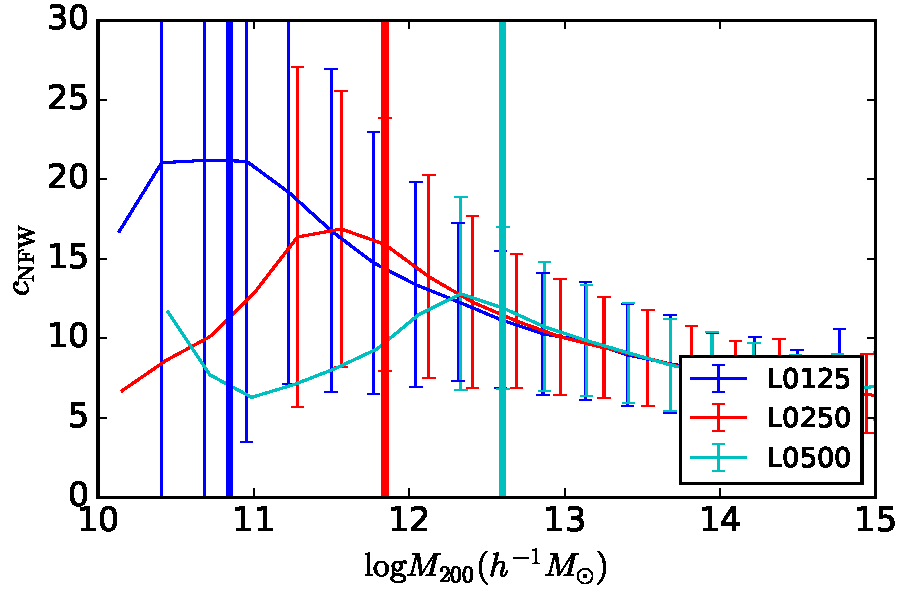
\includegraphics[width=.5\textwidth]{masscut_cNFW_d200.pdf}
\caption{The relationship between the NFW concentration and halo mass for each of our simulations with $\Delta =200$. 
In order of increasing simulation volume, the blue dashed line corresponds to the concentration-mass relation from simulation 
\simA, the red solid line corresponds to \simB, and the cyan dot-dashed line corresponds to \simC. The red error bars show the
dispersion in the values of the mark for \simB. These errors are comparable to those of the other simulations
within the region of interest.
Each simulation is subject to resolution limitations at different halo masses. We show with thick vertical lines 
the minimum $M_{200}$ mass thresholds that we adopt in our analyses using the same color code as 
the concentration-mass relations, going from \simA \ to \simC \ from left to right. Note the deviation from a monotonic trend as a result of resolution effects.}
\label{fig:cnfwrelation}
\end{figure}
%--------------------------------------------------------------------------------


%------------------------------------------ Figure for C_V(M)
\begin{figure}
\centering
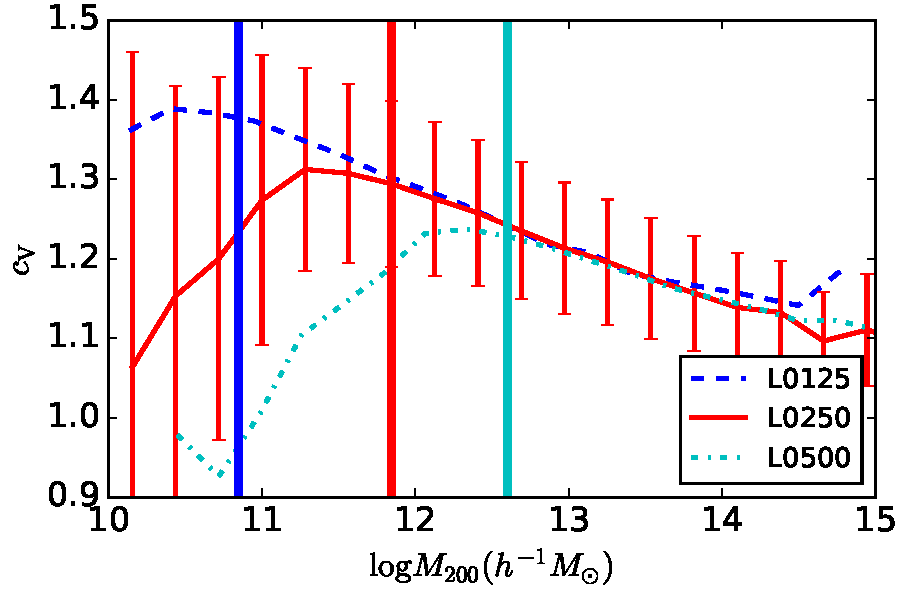
\includegraphics[width=.5\textwidth]{masscut_cV_d200.pdf}
\caption{The relationship between the velocity ratio concentration and halo mass for each of our simulations with $\Delta =200$. 
In order of increasing simulation volume, the blue dashed line corresponds to the concentration-mass relation from simulation 
\simA, the red solid line corresponds to \simB, and the cyan dot-dashed line corresponds to \simC. The red error bars show the
dispersion in the values of the mark for \simB. These errors are comparable to those of the other simulations
within the region of interest.
Each simulation is subject to resolution limitations at different halo masses. We show with thick vertical lines 
the minimum $M_{200}$ mass thresholds that we adopt in our analyses using the same color code as 
the concentration-mass relations, going from \simA \ to \simC \ from left to right. Note the deviation from a monotonic trend as a result of resolution effects.
}
\label{fig:cvrelation}
\end{figure}
%--------------------------------------------------------------------------------

%-------------------------------------------- Figure comparing Cnfw and Cv on a halo-by-halo basis
\begin{figure}
\centering
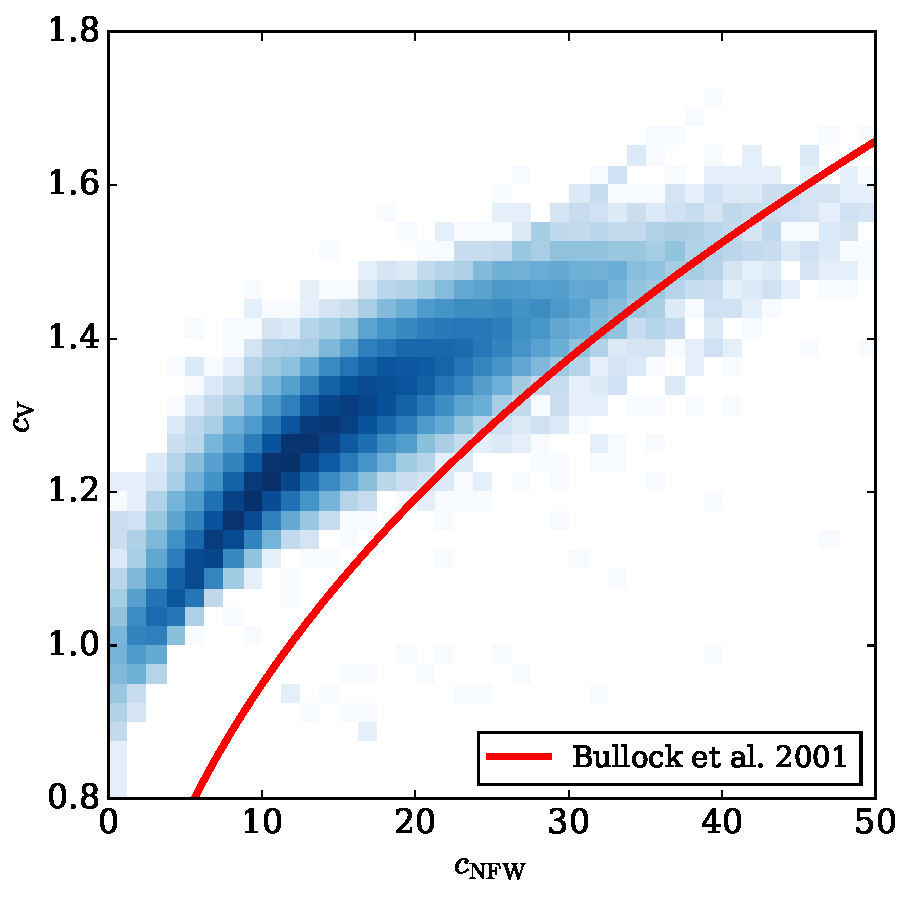
\includegraphics[width=.5\textwidth]{cvvscnfw_relation.pdf}
\caption{
The relationship between the two different marks of concentration, 
using halos in \simB. The color scale, shown at the right, encodes the number of halos 
within a single two-dimensional bin in the $c_{\mathrm{NFW}}$-$c_{\mathrm{V}}$ space. 
The red (blue) regions on the plot show where the most (fewest) halos exist with those values of the two
concentration parameters. The white regions indicate where no halos hold these values. The scatter on this relationship ranges from 5\% for intermediate concentration values, to a high of 13\% at high masses.
}
\label{fig:concentrations}
\end{figure}
%--------------------------------------------------------------------------------------------------------------------------------



In addition to halo concentrations, we examine halo clustering as a function of a variety of other 
halo properties. We study halo clustering as a function of halo shape, $s$, 
quantified by the ratio of the halo minor and major axis lengths, 
%
\beq
s = \frac{c}{a},
\eeq
%
where $a$ is the major axis length and $c$ is the minor axis length. 
The mean relations for halo shapes as a function of halo mass for $\Delta=200$ 
are shown in Figure~\ref{fig:srelation} along with the mass 
thresholds used to ensure that our results are not compromised by 
resolution.


%------------------------------------------ Figure for s(M)
\begin{figure}
\centering
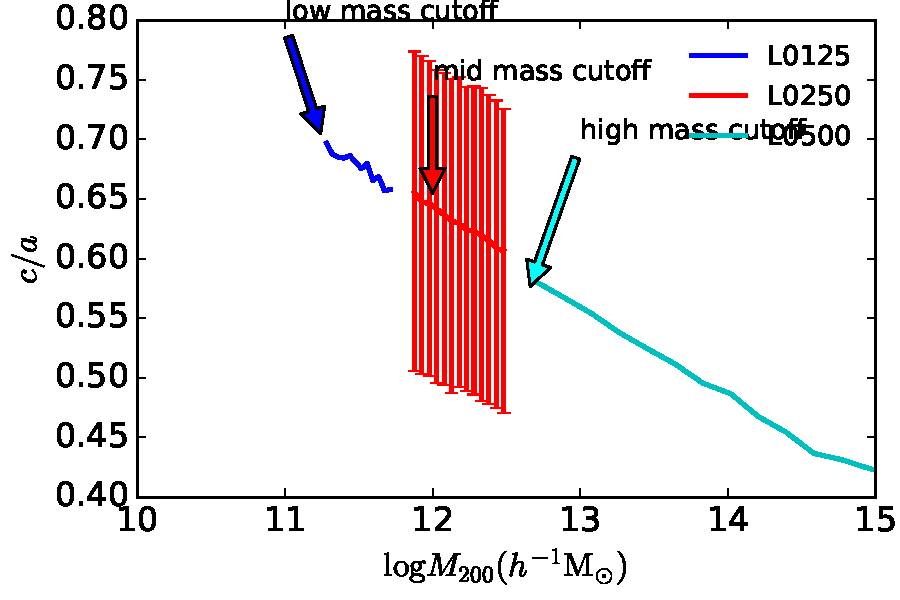
\includegraphics[width=.5\textwidth]{masscut_shape_d200.pdf}
\caption{
The relationship between the halo shape and halo mass for each of our simulations with $\Delta =200$. 
In order of increasing simulation volume, the blue dashed line corresponds to the shape-mass relation from simulation 
\simA, the red solid line corresponds to \simB, and the cyan dot-dashed line corresponds to \simC. The red error bars show the
dispersion in the values of the mark for \simB. These errors are comparable to those of the other simulations
within the region of interest.
Each simulation is subject to resolution limitations at different halo masses. We show with thick vertical lines 
the minimum $M_{200}$ mass thresholds that we adopt in our analyses using the same color code as 
the shape-mass relations, going from \simA \ to \simC \ from left to right. The mass cutoffs chosen for this mark
are at higher masses in order to account for the additional number of particles needed to properly measure the
halo shape. Note the deviation from a monotonic trend as a result of resolution effects.
}
\label{fig:srelation}
\end{figure}
%--------------------------------------------------------------------------------

We study halo clustering as a function of halo angular momentum quantified 
by the spin parameter, $\lambda$, as introduced by \citep{peebles69},
\beq
\lambda = \frac{J \sqrt{\lvert E\rvert}}{G M_{\Delta}^{2.5}}
\eeq
where $J$ is the halo angular momentum, $E$ is the total energy of the 
halo, and $M_{\Delta}$ is the mass at the halo radius, $r_{\Delta}$. 
The mean relations for halo spin as a function of halo mass for $\Delta=200$ 
are shown in Figure~\ref{fig:spinrelation} along with the mass thresholds 
enforced to ensure that our results are not compromised by resolution. 
These thresholds are summarized in Table~\ref{table:thresholds}, where 
we also show the threshold masses at various values of the overdensity 
parameter, $\Delta$.

%------------------------------------------ Figure for lambda(M)
\begin{figure}
\centering
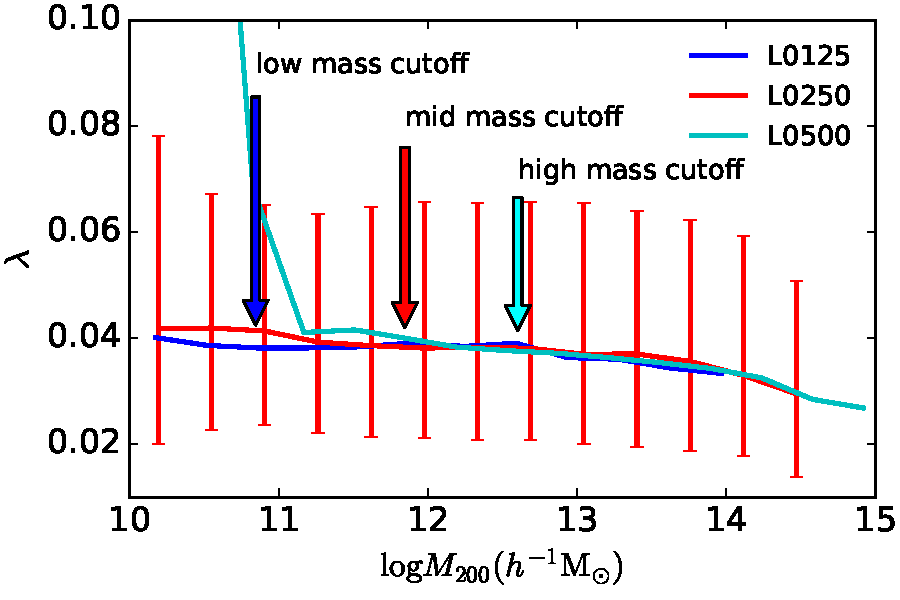
\includegraphics[width=.5\textwidth]{masscut_spin_d200.pdf}
\caption{
\arz{All of the same comments as for Fig.~\ref{fig:cnfwrelation}. Also, there 
is no reason here that the y-axis has to have such a large range. This 
crams all of the data into a small portion of the plot and makes most 
of the plot useless, wasted, white space. A more appropriate y-axis range 
looks to be from -0.1 to about 0.25 or so.}
he relationship between the halo spin and halo mass for each of our simulations with $\Delta =200$. 
In order of increasing simulation volume, the blue dashed line corresponds to the spin-mass relation from simulation 
\simA, the red solid line corresponds to \simB, and the cyan dot-dashed line corresponds to \simC. The red error bars show the
dispersion in the values of the mark for \simB. These errors are comparable to those of the other simulations
within the region of interest.
Each simulation is subject to resolution limitations at different halo masses. We show with thick vertical lines 
the minimum $M_{200}$ mass thresholds that we adopt in our analyses using the same color code as 
the spin-mass relations, going from \simA \ to \simC \ from left to right. Note the deviations from the near linear
trend at low mass due to resolution effects.
}
\label{fig:spinrelation}
\end{figure}
%--------------------------------------------------------------------------------

\arz{I really don't understand what this last paragraph is saying.}
In practice, the mean relations between the various halo properties and the mass thresholds for our analyses 
must be determined separately for each combination of simulation, 
halo property (e.g., $c_{\mathrm{NFW}}$ or $s$), 
and halo definition (the value of $\Delta$ in the case of the present study). 
\arz{The first sentence makes sense and I understand it. It is everything that 
follows that I don't understand. Are you saying that you have a unique threshold 
for each halo property? That is what I get from this statement, but I think that is 
not what you are doing. Can you please clarify this discussion?}
We determine our mass thresholds in order to avoid the regime in which halo parameters
are not well measured due to resolution limits of the simulations; we draw attention to the
downturn in Figure~\ref{fig:cnfwrelation} as an example of this, as the deviation from
the underlying monotonic trend shifts with the change in simulation from low to high mass resolution,
suggesting that this is the result of resolution alone. For ease of comparison
between halo definitions, we choose to use a single mass threshold for each
simulation box size and value of $\Delta$ chosen whenever possible, rather than on a parameter by
parameter basis. This allow for a better comparison as to how the choice of halo
definition impacts each parameter simultaneously, rather than be driven by the
choice of mass cutoff. The one exception to this method is the mass thresholds chosen
for the halo shape parameter. This parameter requires a larger number of particles to be
well measured; we direct attention to the downturn in Figure~\ref{fig:srelation}, which occurs at
an order of magnitude higher mass. We analyze the shape parameter with separate mass thresholds
to maintain the larger number of halos in our sample for the other parameters. This allows us
to have better signal-to-noise in the remaining parameters, while avoiding drawing potentially
erroneous conclusions when analyzing the halo shape parameter.
We summarize the mass thresholds we have used for a 
subset of $\Delta$ values in Table~\ref{table:thresholds}. 
At most values of $\Delta$, the minimum mass thresholds are 
driven by the requirement that the halo properties do 
not suffer significantly from finite resolution effects.
\arz{What else could the thresholds be driven by?}\asv{Uncertain - I cannot think of anything else, now that we
are treating shape as a separate parameter.}


\arz{In the next section, you discuss subhalos. However, in order for the paper to have 
the correct flow, you should introduce the concept of subhalos here and state that we 
will study halo clustering as a function of satellite number.}\asv{Added a section on subhalos when discussing {\tt ROCKSTAR}.
I am unsure if we need to discuss the concept of subhalos here now. That seemed to flow a little better than an
introduction here, since robust identification of halos is a selling point of {\tt ROCKSTAR}.}


\arz{In the table, don't ``low mass," ``mid mass," and ``high mass" correspond to the different simulations? 
For example, low mass corresponds to \simA~and so on? If not, then I don't understand. If so, then you 
should label each cut by the relevant simulation name as well.}
\asv{We use the various mass cuts across simulations, so I was going for a more general name - e.g., 
we use high mass on both L0250 and L0500, which allows us to probe if the relation is driven by the 
simulation size or the actual mass threshold. I can swap out to more specific names though, but I 
thought that might cause confusion. It seems like we have swapped away from that methodology 
in the final version, so that might be best.}
\arz{I still prefer using the simulation name to specify the threshold, 
otherwise the name seems arbitrary.}\asv{Switched to using halo name and a tag.}


%%%%%%%%%%%%%%%%%%%%%%%%%%%%%%%%%%%%%%%%%%%%%%%%%%%%%%%%%%%%%%%%%%%%%%%%%%%%
\begin{table*}
\caption{
Minimum mass thresholds for each of our analyses depending upon the 
value of the overdensity, $\Delta$, used to define the halos. 
In the columns below the values of $\Delta$ we show the minimum 
host halo masses considered in units of $h^{-1}\mathrm{M}_{\odot}$.
Those rows without a label of '-shape' refer to the mass cut chosen for all parameters other than
halo shape. Those rows with a label of '-shape' refer to the mass cut chosen for the shape parameter.
The latter requires a higher mass cut due to the larger number of particle required in order to have a
robust measurement of halo shape.}
\vspace*{8pt}
\begin{tabular}{ c c c c c c c }
\hline
\hline
Cutoff Name &  $\Delta=340$ & $\Delta=200$ & $\Delta=100$ & $\Delta=75$ & $\Delta=50$ & $\Delta=10$ \\
\hline
\\{low mass} & {N/A} & $7 \times 10^{10}$ & $8 \times 10^{10}$ & $9 \times 10^{10}$ & $1 \times 10^{11}$ & $2 \times 10^{11}$  \\
{low mass-shape} & {N/A} & $1 \times 10^{11}$ & $1 \times 10^{11}$ & $1 \times 10^{11}$ & $1 \times 10^{11}$ & $1 \times 10^{11}$ \\
{mid mass} & {N/A} & $7 \times 10^{11}$ & $8 \times 10^{11}$ & $9 \times 10^{11}$ & $1.5 \times 10^{12}$ & {N/A} \\
{mid mass-shape} & {N/A} & $1 \times 10^{12}$ & $1 \times 10^{12}$ & $1 \times 10^{12}$ & $1 \times 10^{12}$ & {N/A} \\
{high mass} & $3 \times 10^{12}$ & $4 \times 10^{12}$ & $5 \times 10^{12}$ & $6 \times 10^{12}$ & $7 \times 10^{12}$ & {N/A} \\
{high mass-shape} & $1 \times 10^{13}$ & $1 \times 10^{13}$ & $1 \times 10^{13}$ & $1 \times 10^{13}$ & $1 \times 10^{13}$ & {N/A} \\
\hline
\hline
\end{tabular}
\label{table:thresholds}
\end{table*}
%%%%%%%%%%%%%%%%%%%%%%%%%%%%%%%%%%%%%%%%%%%%%%%%%%%%%%%%%%%%%%%%%%%%%%

\arz{I would like to see another figure here. I would like to see $M_{200}$ on the x-axis and $M_{\Delta}$ on the y-axis. What should be plotted is the mean $M_{\Delta}$ as a function of $M_{200}$ for all halos common to both catalogs. This will be a nice informative plot for the reader and will help the reader to digest the table.}
\asv{Will do using the halo matched catalogs - in progress.}

%-----------------------
\section[]{Halo Clustering as a function of Auxiliary Halo Properties}
\label{section:methodology}
%-----------------------

%----------------------------------------------------------
\subsection{Auxiliary Halo Properties}


We are interested in studying the clustering behavior of halos as a function of 
properties other than mass. As mass is the dominant halo property determining halo
clustering strength and environment, we refer to the other properties that we study as 
``auxiliary halo properties" (those properties other than mass, such as concentration 
$c_{\rm NFW}$ or shape $s$). As has been demonstrated extensively in the literature, 
the auxiliary properties that we consider are a function of mass \citep{bullock_etal02,allgood_etal06, duffy_etal08, despali_etal16}. 
\arz{Cite the Bullock et al. (2001) paper on halo concentrations here. Also, search to see if there are 
other papers with mass dependences of the other parameters. There probably will be and we probably 
need more citations here.} 
This mass dependence induces auxiliary-property-dependent halo clustering. 
Most contemporary cosmological $N$-body simulations, and specifically the suite of simulations 
that we study in this work, do not have a sufficiently large number of halos to make isolating halos 
of fixed mass, and then further splitting these halos by an auxiliary property, a powerful method with 
which to study the dependence of clustering on auxiliary properties. Therefore, it is 
necessary to remove or mitigate the mass dependence of the auxiliary properties that we 
study. 

We mitigate the mass dependence of the auxiliary properties as follows. First, 
we take all host halos more massive than our minimum mass thresholds and sort them by 
their halo masses, $M_{\Delta}$. We place these halos into ten logarithmically-spaced bins 
of halo mass, ensuring that no bin has fewer than XXX halos. 
\arz{I was under the impression that you used the median value? Can you 
check on this.}\asv{Currently we are using the mean - as I recall this does not
create any significant difference in result. Perhaps I should add a line though
suggesting that our method is robust with choice of summary statistic here? We also
do not currently have a hard bin number cutoff. Ten was just chosen such that each
bin has at least a few halos in it.}
The mean value of each halo property is calculated within each bin, 
and subtracted from the recorded value for each halo in the bin. 
This removes the strong mass trend in each of these properties. 
We use these new measures of halo auxiliary properties, those with 
the mean mass trend removed, to study halo clustering strength 
in the remainder of this work.
\arz{You should make sure that your results do not change qualitatively 
under a few modifications. First, make sure that if you use finer binning 
that nothing qualitative changes (small quantitative changes can be acceptable). 
We have to be sure that our results are not sensitive to the number of bins 
that you choose here. Second, you should make sure that your results are 
not qualitatively different if you use medians rather than means. Third, 
I believe that you also explore removing the mass trend by removing 
a best fit power law $c(M)$ (or $s(M)$ or $\lambda(M)$ or whatever) relationship?
If so, that is great. You should conclude this sentence with a statement along 
the lines of ``We have experimented with a variety of methods to remove the 
gross mass dependence of these auxiliary properties and have verified that 
our qualitative results are not sensitive to the number of bins we use or the 
choice of median or mean property. Further, we have experimented with 
removing the gross mass dependence of auxiliary halo properties by subtracting 
away a best-fit power law relation for the property of interest and again, we 
find that our qualitative results are not altered using this method." We have 
to be able to give the reader some sort of confidence that our results are not 
driven by these seemingly arbitrary choices.}
\asv{I'm not necessarily comfortable with the current ten bin situation and could conceivably switch back to equally populated bins, which allows for more total bins with halos to look at, but unevenly spaced in log mass.}
\arz{You should do whatever is most robust. Using either method, you should choose sufficiently large number of 
bins that our primary results are not altered by changing the number of bins.}



\arz{Flesh this out a bit. See the discussion in Wechsler et al. 06 as a model. 
The specific values of the thresholds need to be given} 
\asv{Slight change - following Wechsler et al 06 does not ever put a specific limit on 
subhalo velocity and instead places a limit on the ratio between the subhalo velocity and 
the host velocity as the prime limit. Just making sure that lines up well.}


Host halo size and the number of satellite halos 
(above some threshold in a proxy of satellite halo size) are also strongly correlated. 
To mitigate the correlation between halo mass and abundance of subhalos, 
we follow the prescription of \citet{wechsler_etal06}. First, we select host halos 
with $v_{\mathrm{max,host}} \ge 240 \ \mathrm{km \ s}^{-1}$. This ensures that the satellite counts 
will be minimally affected by finite resolution. We then select subhalos
from the sample based on the criteria that the ratio $V_{\mathrm{max,sub}}/V_{\mathrm{max,host}} \ge 0.3$, 
where $V_{\mathrm{max,sub}}$ and $V_{\mathrm{max,host}}$ are the maximum circular velocities 
of the subhalos and host halos respectively. This scaling exploits the fact that the subhalo velocity 
function is a very nearly self-similar function \citep{zentner_etal05}[and references therein], 
so that scaling subhalo $V_{\mathrm{max,sub}}$ by host $V_{\mathrm{max,host}}$ 
eliminates the gross mass dependence of satellite number. The threshold value for this velocity ratio was chosen 
such that all host halos that make the above cut contain, on average, more than one satellite halo. 
Subhalo maximum circular velocities were used as a proxy for subhalo size rather than subhalo masses because 
subhalo maximum circular velocities can be more robustly measured from simulation data, making 
comparison to other work easier.


%---------------------------------------------------------------
\subsection{Clustering Statistics}
%---------------------------------------------------------------


We assess the influence of assembly bias on two-point statistics of host halos. In order to do so, we 
study both the standard two-point correlation functions of halos selected by properties other than mass 
(e.g., the auxiliary properties concentration, shape, and spin) as well as halo mark correlation functions
(MCFs). MCFs quantify the manner in which a halo property (the ``mark") correlates among halo pairs as a function
of the distance between the pairs. MCFs have the advantage that they effectively stack signal from all values of 
the halo auxiliary property, or mark, in contrast to selecting subsets of halos based on the auxiliary property and 
MCFs stack signal from all environments and do not require any specific definition of halo environment in order 
to detect environmental trends. Absent halo assembly bias, the halo marks are uncorrelated among pairs. 
MCFs have been used in many previous papers to quantify environmental dependence of halo 
properties other than mass \citep{sheth_tormen04,sheth05, harker_etal06,wechsler_etal06,mao_etal15} \arz{I think there are also a couple of 
Sheth papers that should be cited here, maybe more. Check on that.}\asv{Think I got the most relevant Sheth papers here now.}. 


For a specific halo property, or mark $m$, we use the MCF normalization of \citet{wechsler_etal06}, namely 
%
\beq
\mathcal{M}_m(r) \equiv ( \langle m_1 m_2 \rangle_p (r) - \langle m \rangle^2 / \mathcal{V}(m),
\eeq
%
where $m_{\mathrm{i}}$ is the value of the mark for halo $\mathrm{i}$, $\langle m \rangle$ is the mean of the
mark, and $\mathcal{V}(m)$ the variance of the mark. The notation is intended to indicate that the average is
taken over all pairs of halos separated by a distance $r$. In the absence of any correlation between a halo
property among neighbors a separation $r$ away, $\mathcal{M}_m(r) = 0$. Deviations of the MCF from
zero indicate such correlations exist and the size of the $\mathcal{M}_m(r)$ gives the excess of the mark among
pairs compared to the one-point mean of the mark $\langle m\rangle$ in units of the one-point variance. 


It is necessary to assess statistical fluctuations in the statistics that we measure in these simulations in
order to determine the significance of the signals. For two-point correlation functions, we determine the
covariance of the measurement through jackknife resampling of the eight octants of the simulation cube. We assess
the statistical significance of the MCFs by randomly re-assigning each of our marks to the halos in the sample. 
We then compute the MCF of these randomized marks. As the mark re-assignment is random, 
the MCF computed on these re-assigned marks {\em cannot} exhibit any 
environment dependence other than that induced by statistical fluctuations. 
We perform this reassignment 400 times and approximate a $2\sigma$ error region by 
the span of the MCF between our 10$^\mathrm{th}$ lowest and 10$^\mathrm{th}$ highest (that is the
390$^\mathrm{th}$ if the MCFs were sorted in ascending order) values of the MCF. In the event that there are no
environmental correlations with halo auxiliary properties, the MCFs measured in the simulations would fall within
this error band $95\%$ of the time. 


%----------------------------
\section[]{Results}
\label{section:results}
%----------------------------


%-----------------------------------------------
\subsection{Correlation Functions}
\label{sub:cfresults}

\arz{Fix up and fill in numbers as needed, but follow this general format.}
We begin by studying the correlation functions of halos in our mass threshold samples, sub-selected by auxiliary
properties. Figure~\ref{fig:cc_cfcompare} exhibits the difference between the clustering strength of halos in the
$20^{\mathrm{th}}$ percentile highest NFW-defined halo concentrations and the halos with the halos that have the
$20^{\mathrm{th}}$ percentile lowest NFW-defined halo concentrations as a function of the overdensity parameter, $\Delta$, used to
define the halos and normalized by the clustering strength of the entire halo
sample. \arz{which concentration?}\asv{Not sure if I should refer to them as NFW-defined concentration or NFW concentrations.} 
If the clustering strength of halos was independent of halo concentration, we 
would expect these lines to cluster around zero. The witnessed deviation
demonstrates that halos of different NFW-defined halo concentration exhibit appreciably different clustering. \arz{How can you make a statement about auxiliary properties 
in general, when you only plot concentration?}\asv{I agree that I cannot: got ahead of myself in the writing.}
Furthermore, it is clear that the strength and sign of assembly bias due to NFW-defined halo concentration is 
strongly mass dependent for any fixed halo definition, 
a result that agrees with the significant previous literature on halo assembly bias using conventional halo definitions 
\citep{wechsler_etal02, gao_etal05, zentner07, wechsler_etal06, harker_etal06, croton_etal07, dalal_etal08, mao_etal15, sunayama_etal16}\arz{Cite all the usual 
papers here, Gao, Wechsler, Harker, Zentner07, Dalal07, probably several more.}\asv{I think that is most of the
usual suspects, but I'll do a double check for more important ones!} 
At relatively low mass (the low mass panel, 
$M_{200} > 7 \times 10^{10} \hMsun$), high-concentration halos are considerably 
more strongly clustered than low-concentration halos using the more 
conventional $\Delta = 200$ definition for halos. At somewhat higher halo masses 
(the mid mass panel, $M_{200} > 7\times 10^{11} \hMsun$), this difference is markedly reduced. 
Finally, for the highest mass halos that we have
the capability of studying (the high mass panel, $M_{200} > 4 \times 10^{12} \hMsun$), 
the effect is of opposite sign; low-concentration halos are more strongly correlated 
than high-concentration halos.


Focus first on the middle panel of Fig.~\ref{fig:cc_cfcompare}. In this panel, corresponding to the 
mid mass threshold, the difference in large-scale clustering between high- and low-concentration halos 
is dramatically reduced for a halo definition with $\Delta=75$. Further decreasing $\Delta$ leads to
concentration-dependent clustering of opposite sign. Comparing the differing clustering 
strengths across the three panels of Fig.~\ref{fig:cc_cfcompare}, it is clear that this is not a universal
conclusion. For low-mass halos (the top panel), very low values of $\Delta$ (and correspondingly large definitions of halo radii,
as $R_{\Delta} \propto \Delta^{-1/3}$) are necessary in order to mitigate the concentration dependence of halo
clustering. Conversely, for higher
mass halos (the bottom panel), values of $\Delta \approx 200$ yield little concentration-dependent clustering. In
this case, decreasing $\Delta$ (increasing $R_{\Delta}$) results in significantly {\em increased} concentration
dependent halo clustering. The reasons for these changes are of interest and we return to the interpretation of 
these results below.

Notice that in all panels of Fig.~\ref{fig:cc_cfcompare}, the effect of concentration-dependent clustering is
scale-dependent. Moreover, the effect is scale-dependent for all values of $\Delta$. In these cases, simply
defining halos with a different value of $\Delta$ does not suffice to eliminate concentration-dependent
clustering on all scales. In this discussion and throughout, we focus primarily on the large scale clustering,
which we take to mean clustering on scales significantly larger than the radii, $R_{\Delta}$ of the halos in our
samples.


%---------------------------------------------------------------------------------------------------------------------------------------
\begin{figure}
	\centering
	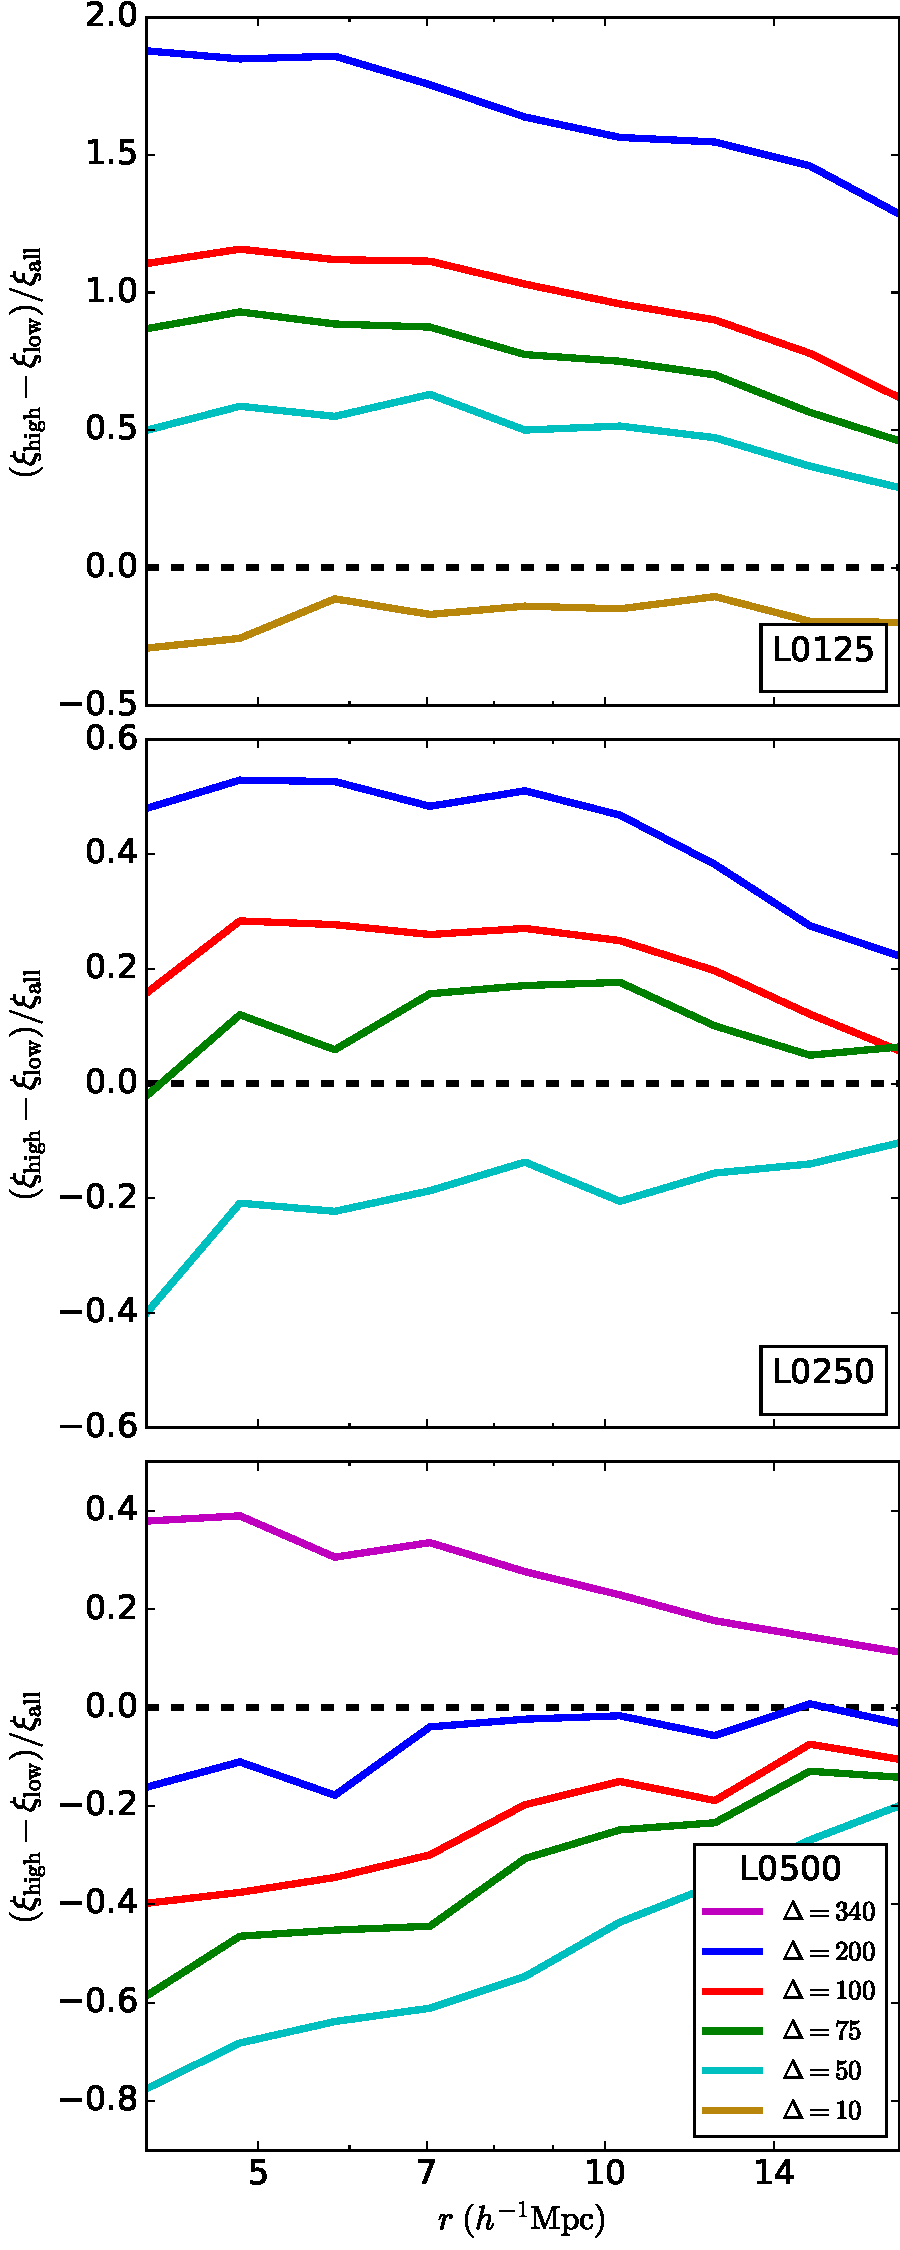
\includegraphics[width=.4\textwidth]{all_cfcompare_cnfw.pdf}
	\caption{
In each panel, the solid lines plot the difference between the correlation function for the top
20\% and the bottom 20\% of halos as determined by NFW-defined concentration, normalized by the
correlation function of the entire sample. In each plot the line with the most positive value
corresponds with the largest value of overdensity parameter, $\Delta$, and demonstrates a smooth
trend down to the lowest value of $\Delta$. The top (middle/bottom) panel shows the results for the
\simA \ (\simB /\simC) data set utilizing the low mass (mid mass/high mass) cutoffs. Note
that the top panel is the only one where exploring the extreme regime of $\Delta = 10$ is
necessary, while the bottom panel is the only one where the exploration of $\Delta = 340$
is necessary.}
\arz{You need to describe each line type in the panels.}
\asv{May still need error bars, depending on how clean we want the overall image, but should be quick enough to whip together.}
\arz{For errors, you don't want the jackknife error bars. What you want is to show the range you get when you randomly 
sub-sample 20\% of all halos repeatedly.}\asv{This is currently not in the
analysis pipeline. Running marked correlation functions handles the
randomization runs on its own. I'm going to finish the existing runs
in order to get data to work with for the other plots and then I will
look into rewriting this set of plots using the marked correlation function
code with a weight of 1 so I can take advantage of the random error routine
built into it. That still leaves the question of how the error should be
shown on this figure - it is the correlation function of the high fraction
minus the correlation function of the low fraction normalized by the
correlation function of the entire sample. We would have individual
sample errors w/ high and low points, but how do I plot the error range on
this? Largest difference between the two samples? Median difference?}
\label{fig:cc_cfcompare}
\end{figure}
%----------------------------------------------------------------------------------------------------------------------------------------------

\arz{I assume that if you made the same plot for $c_V$ we would reach the same basic conclusions as for $c_{NFW}$? If this is so, then you need to add a specific statement in this regard to the end of the discussion above. In this case, no new figure would be needed. If not, then you need to show the figure.}
 
 \arz{You need to make some statement that the same conclusions would be reached with $c_{\mathrm{V}}$.}
 
 \arz{In this subsection, I advocate at least one and perhaps two new figures. First, can you make an analogous plot to Fig.~\ref{fig:cc_cfcompare} that shows some other property, such as shape or spin? This would be a nice addition for completeness. Second, what would happen if you used 50\% or 10\% cuts on concentration? Would we reach nearly the same conclusions? If so, then you do not need to show the plots explicitly. However, in this case, you DO need to state explicitly that this is the case. In other words, you need to state the the broad conclusions we reach are roughly independent of the specific percentiles that we use to select halos so that showing results for a variety of different percentiles doesn't add very much to the discussion. It is also possible that selecting on a different percentile yields an entirely different conclusion. I don't suspect that this will be the case, but it is possible. If that happens, then you need to show an example of such a figure for, say, concentration.}
\asv{These have all been tested at this point. They do not offer any unique conclusions, so I am uncertain if they want to be included beyond the concentration one, which shows the equivalence of the two methods.}

\arz{If you have tested these things, then you really need to have a paragraph in here at this point stating 
that you've checked these things and that they do not lead to any significantly different conclusions.}
\asv{Going to rerun these tests as soon as the new data pipeline finishes
running as a final confirmation just to make certain. Adding in the section
now though.}

It should be noted that this method is robust to the choice of sample cut;
changing from 20\% cut on NFW-defined concentration to a 50\% or 10\% cut on
NFW-defined concentration does not change the conclusions that we draw from
Fig.~\ref{fig:cc_cfcompare}. Furthermore, we note that the conclusions drawn
from these methods are equivalent to those drawn in \ref{sub:mcfresults}
below. As the method described in that section has a better measured signal
and has proven to have equivalent results, we choose to focus our efforts on
that methodology.
\asv{trying to think of how to word the fact that we focus on the MCF as a
better measurement than the correlation function comparison, but I'm failing
to think of the best way to word that.}

%-----------------------------------------------------------------
\subsection{Mark Correlation Functions}
\label{sub:mcfresults}

\begin{figure}
	\centering
	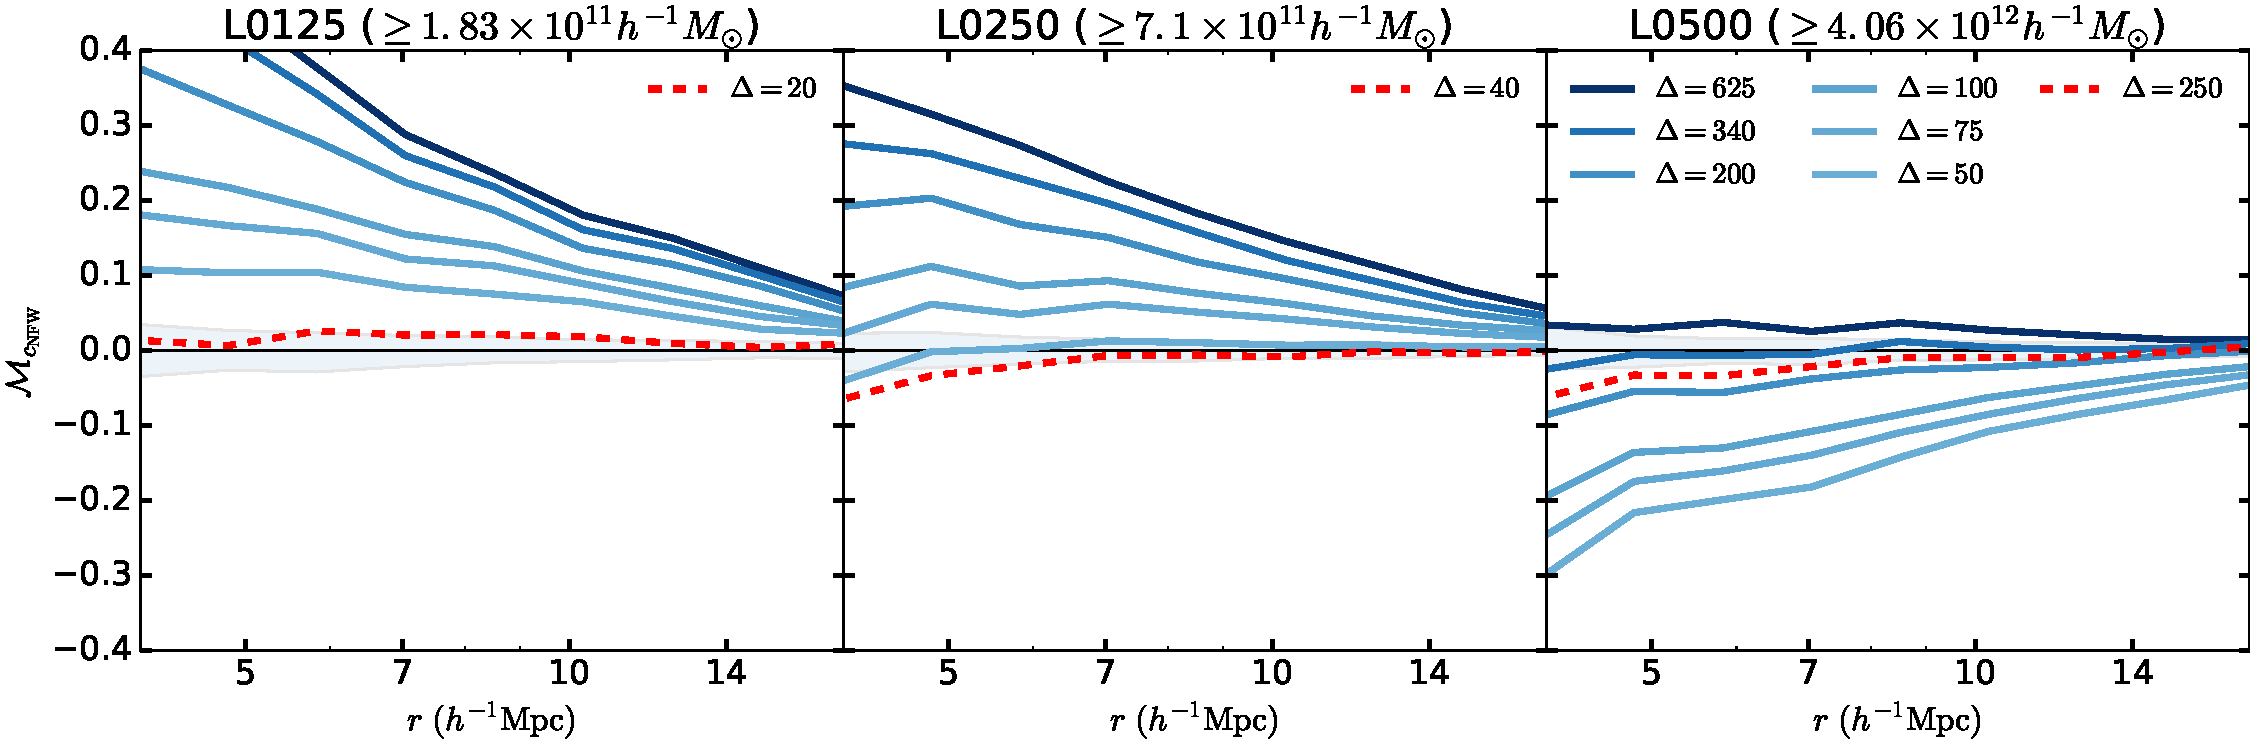
\includegraphics[width=.4\textwidth]{all_mcf_cNFW.pdf}
	\caption{
The marked correlation function for the concentration defined according to the 
NFW profile. The solid lines plot the marked correlation function using NFW-defined concentration as the mark. In each plot the line with the most 
positive value corresponds with the largest value of overdensity parameter, 
$\Delta$, and demonstrates a smooth trend down to the lowest value of 
$\Delta$. The top (middle/bottom) panel shows the results for the
\simA \ (\simB /\simC) data set utilizing the low mass (mid mass/high mass) cutoffs. Note
that the top panel is the only one where exploring the extreme regime of $\Delta = 10$ is
necessary, while the bottom panel is the only one where the exploration of $\Delta = 340$
is necessary. The shaded bands represent 2-sigma confidence regions generated by randomization of the marks.
}
	\label{fig:cc_mcf_cnfw}
\end{figure}


We now move toward a discussion of halo assembly bias as diagnosed by MCFs. 
MCFs have the advantage that it is not necessary 
to specify particular auxiliary property subsamples, such as the percentiles above, 
in order to assess assembly bias.\footnote{Of course, this comes at the cost of averaging 
over all values of the auxiliary properties. Using MCFs it is not evident if the assembly bias effect is a smooth
function of the auxiliary property, dominated by the tails of the auxiliary property, or has some more complex
dependence upon the auxiliary property. Our results in \S~\ref{sub:cfresults} suggest that assembly bias is a
fairly smooth function of the auxiliary properties.} 
The NFW concentration, $c_{\mathrm{NFW}}$, MCF is shown in Figure~\ref{fig:cc_mcf_cnfw}. 
The shaded bands in the figure delineate the statistical fluctuations in MCFs induced by 
finite sampling as discussed in the previous section. Qualitatively, 
Fig.~\ref{fig:cc_mcf_cnfw} exhibits the same features that are evident in 
Fig.~\ref{fig:cc_cfcompare}: more concentrated halos are significantly more clustered in 
the low-mass L0125 halo sample; concentration-dependent halo clustering weakens and 
reverses sense as halo mass increases, consistent with work on assembly bias by \citet{sunayama_etal16}; for the 
L0250 sample with $\Delta=75$, the large-scale concentration dependence of halo clustering has been reduced so as to 
be consistent with zero within the statistical limitations of the simulation. \arz{It seems like we need 
$\Delta \sim 65-70$ for L0250?}\asv{We have (or will have) the data from
$\Delta = 70$, though it is not currently plotted due to cleanliness. I could
always drop the $\Delta = 75$ in favor of it across the board.}


Figure~\ref{fig:cc_mcf_cV} is a similar plot for the velocity-defined concentration, $c_{\mathrm{V}}$ MCF. 
This figure exhibits qualitatively and quantitatively similar features to Fig.~\ref{fig:cc_mcf_cnfw}, a 
fact that is not surprising given that we already know that $c_{\mathrm{NFW}}$ and $c_{\mathrm{V}}$ 
quantify largely redundant information about their halos.

%---------------------------------------------------
\begin{figure}
	\centering
	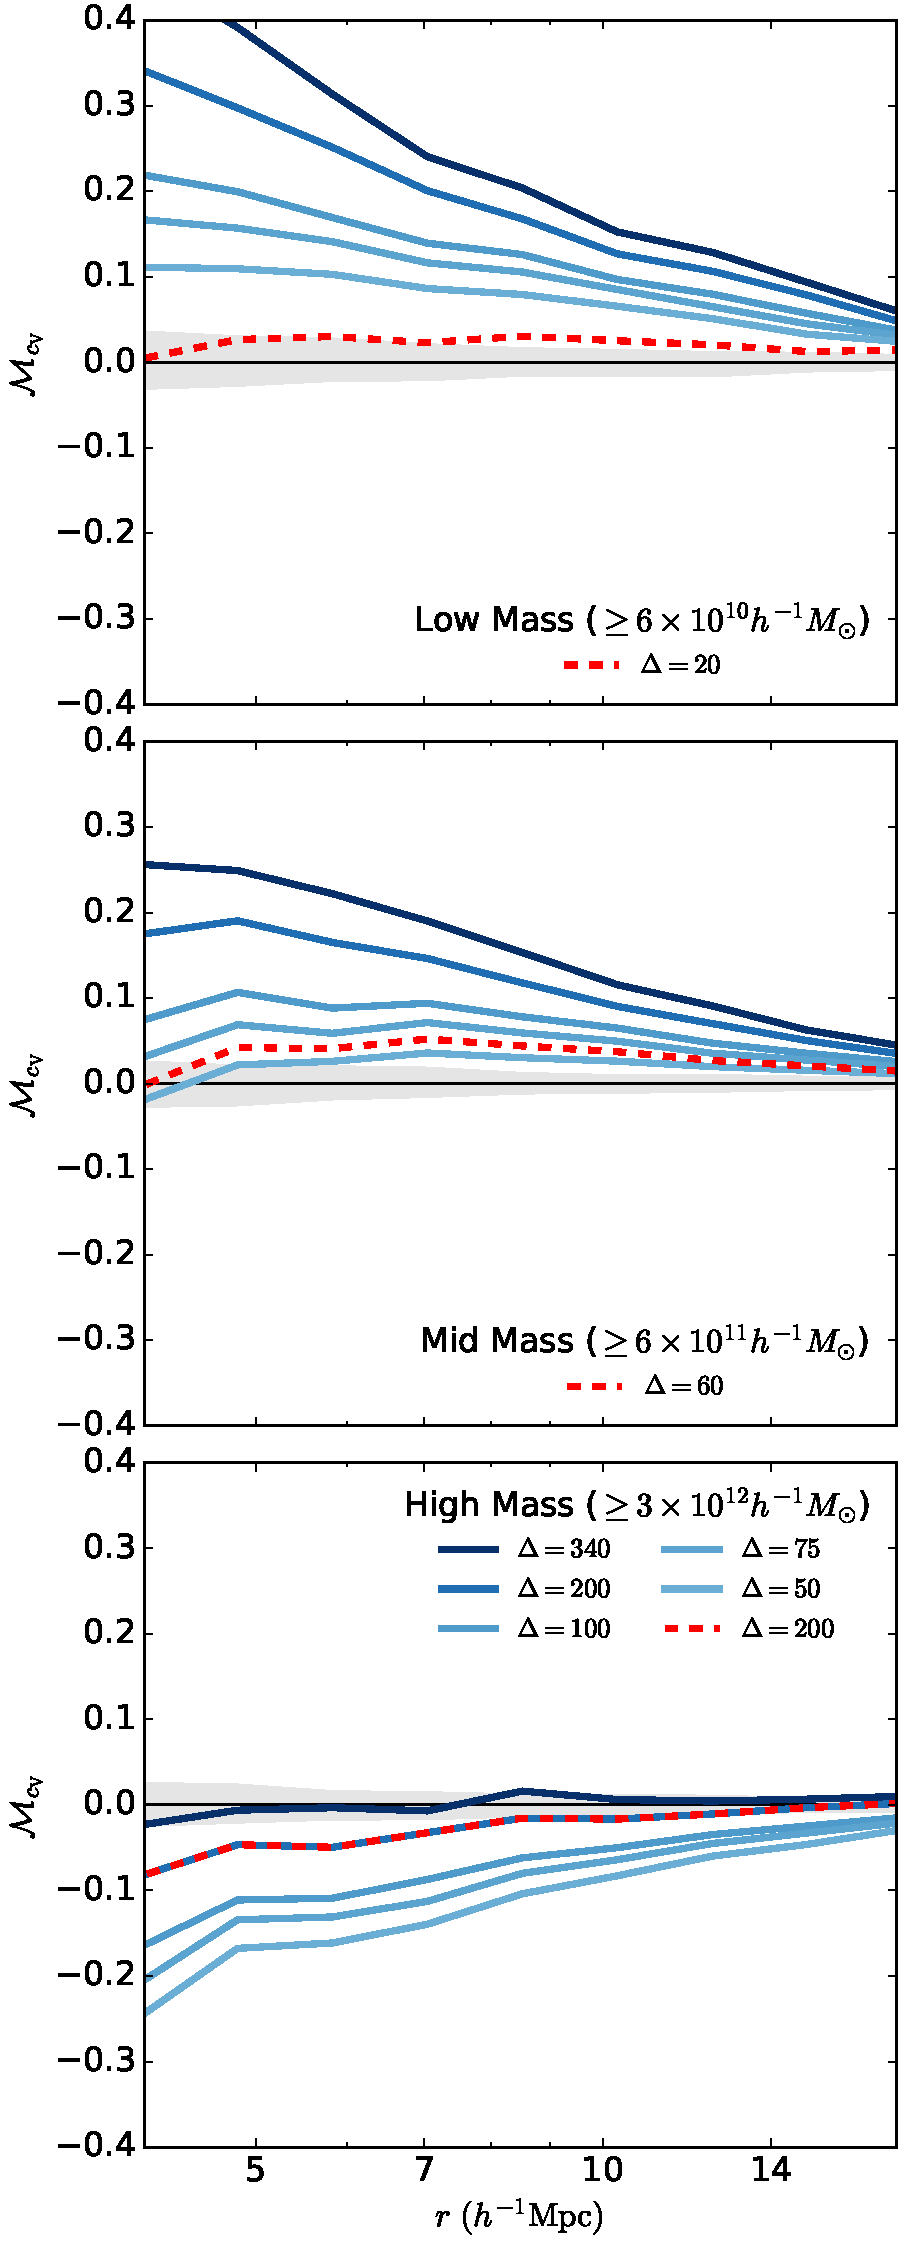
\includegraphics[width=.4\textwidth]{all_mcf_cV.pdf}
	\caption{The marked correlation function for the concentration defined according to the ratio of max circular velocities. The solid lines plot the marked correlation function using velocity ratio concentration as the mark. In each plot the line with the most 
positive value corresponds with the largest value of overdensity parameter, 
$\Delta$, and demonstrates a smooth trend down to the lowest value of 
$\Delta$. The top (middle/bottom) panel shows the results for the
\simA \ (\simB /\simC) data set utilizing the low mass (mid mass/high mass) cutoffs. Note
that the top panel is the only one where exploring the extreme regime of $\Delta = 10$ is
necessary, while the bottom panel is the only one where the exploration of $\Delta = 340$
is necessary. The shaded bands represent 2-sigma confidence regions generated by randomization of the marks.
}
	\label{fig:cc_mcf_cV}
\end{figure}
%---------------------------------------------------

Moving on from concentrations, Figure~\ref{fig:cc_mcf_s} illustrates MCFs in which the mark is the shape
parameter, $s$, of the halo. The environmental dependence of shape parameter is distinct from that of
concentration in a number of ways. Notice that at all masses and at all halo definitions, less spherical halos
(halos with smaller $s$) are more strongly clustered. Furthermore, decreasing $\Delta$ (increasing halo radius)
only serves to increase this environmental dependence in all cases. This is indicative of halo shapes being
driven by structure on scales larger than halo radii, in particular $R_{200}$, and is not entirely surprising
given our significant amount of knowledge of the filamentary nature of large-scale structure. We note that while
there is a change from this trend for the smallest values of $\Delta$ studied, the extreme choice of $\Delta$ does
seem to mark a reversal in this trend. We examine this possibility in Figure~\ref{fig:matched_shapecomp},
which compares the mean measured halo shape in equally spaced bins of log halo mass, along with their mean
dispersion. The methodology of halo matching is discussed below.

We note that the dispersion in halo shape remains quite similar, though the average halo becomes more
circular. Due to the nature of our method of halo redefinition and the lack of a clear trend in the halo shape
marked correlation function, it is difficult to draw definitive conclusions as to the nature of this result.
\asv{I feel that the $\Delta=10$ shape is questionable given the extreme value of $\Delta$, but there does not
seem to be anything that is a smoking gun as to why it is wrong. It seems counterintuitive to me as well, as
I thought the use of high values of $\Delta$ was to deal with the core of the halo which would be more spherical
on average, while this seems to suggest the trend is opposite. Thoughts on this are much appreciated. Also,
I feel I should move this further in, perhaps with the other matched catalog comparison?}
\begin{figure}
	\centering
	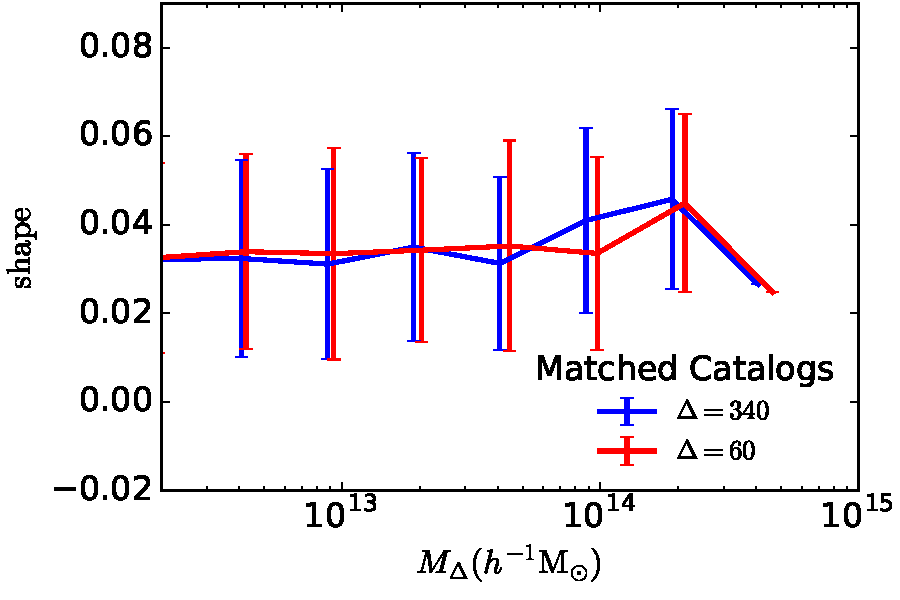
\includegraphics[width=.4\textwidth]{matched_catalog_shapecomp.pdf}
	\caption{A comparison of the mean value of the halo shape for halos matched across both
	the $\Delta = 200$ and $\Delta = 70$ catalogs for \simB. The blue (red) line shows the mean value and scatter of
	the	mean for the $\Delta = 200$ ($\Delta = 70$) catalog. Note that there is no significant
	increase in the scatter of the mean due to the change in halo definition.}
	\label{fig:matched_shapecomp}
\end{figure}
\arz{If possible, a
line here with $\Delta \gg 200$. Seems like it could be instructive, let me know if this is going to take a long
time or be very onerous.}\asv{Added and continues the trend in the direction as expected. Note reversal in
monotonic relationship for lowest mass objects though. Looking over the cuts, this may imply that the mass cuts
are not aggressive enough for the shape mark, though. Vega et al 2016 paper suggests this is the case.}


The spin MCFs are shown in Figure~\ref{fig:cc_mcf_spin}. Qualitatively, spin-dependent halo clustering is 
quite similar to shape-dependent halo clustering. Halos of high-spin cluster more strongly than halos of 
low-spin. \arz{Search the literature, particularly Brandon Allgood's papers and Andreas Faltenbacher whose 
names come to mind, for spin-dependent assembly bias. I'm trying to figure out if yours is the first paper 
to point this out.}\asv{Need to track down all the specific citations, but after changing our normalization
method, it seems to match up better with existing texts.} Likewise, increasing halo radii by decreasing $\Delta$
in halo definitions only drives spin-dependent halo clustering to be stronger.

%---------------------------------------------------
\begin{figure}
	\centering
	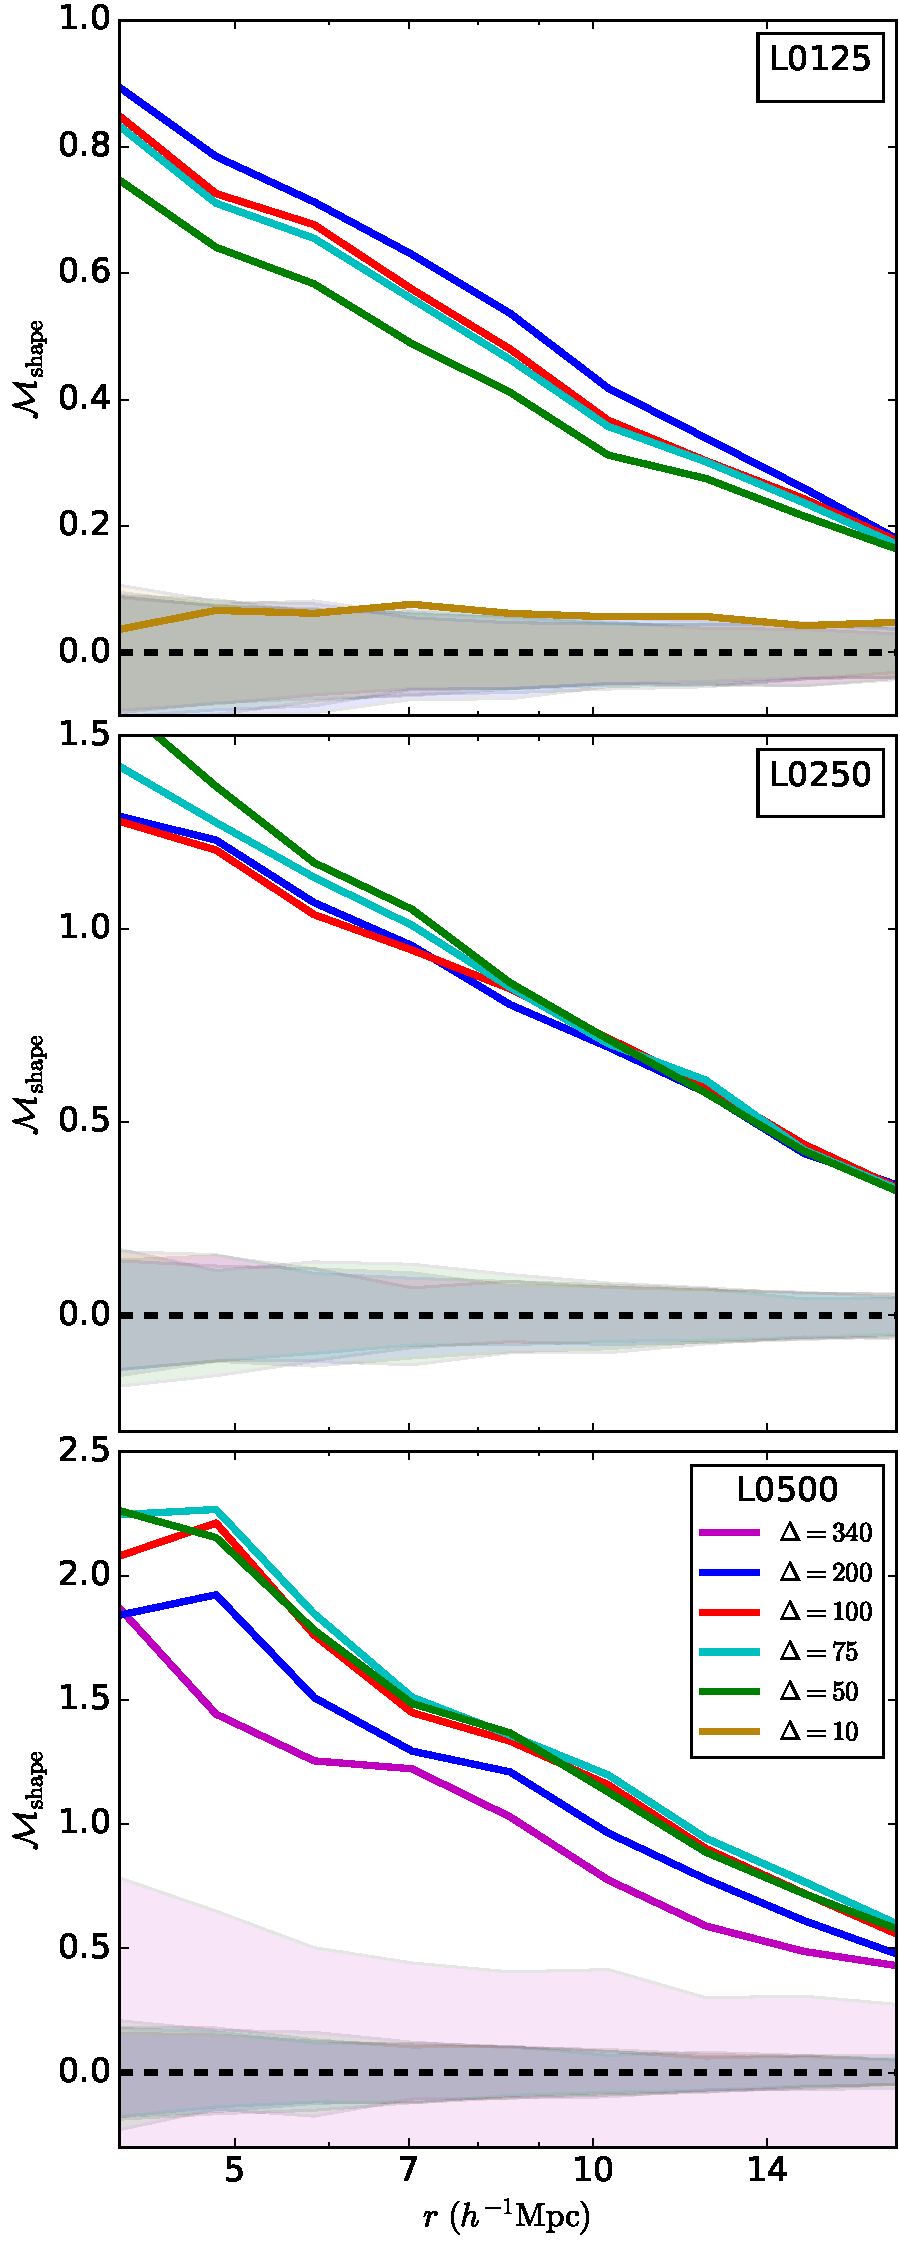
\includegraphics[width=.4\textwidth]{all_mcf_shape.pdf}
	\caption{
	The marked correlation function for the halo shape parameter. The solid lines plot the marked correlation function using halo shape as the mark. The top (middle/bottom) panel shows the results for the
\simA \ (\simB /\simC) data set utilizing the low mass-shape (mid mass-shape/high mass-shape) cutoffs. Note
that the top panel is the only one where exploring the extreme regime of $\Delta = 10$ is
necessary, while the bottom panel is the only one where the exploration of $\Delta = 340$
is necessary. The shaded bands represent 2-sigma confidence regions generated by randomization of the marks.}
	\label{fig:cc_mcf_s}
\end{figure}
%--------------------------------------------


%---------------- spin MCF
\begin{figure}
	\centering
	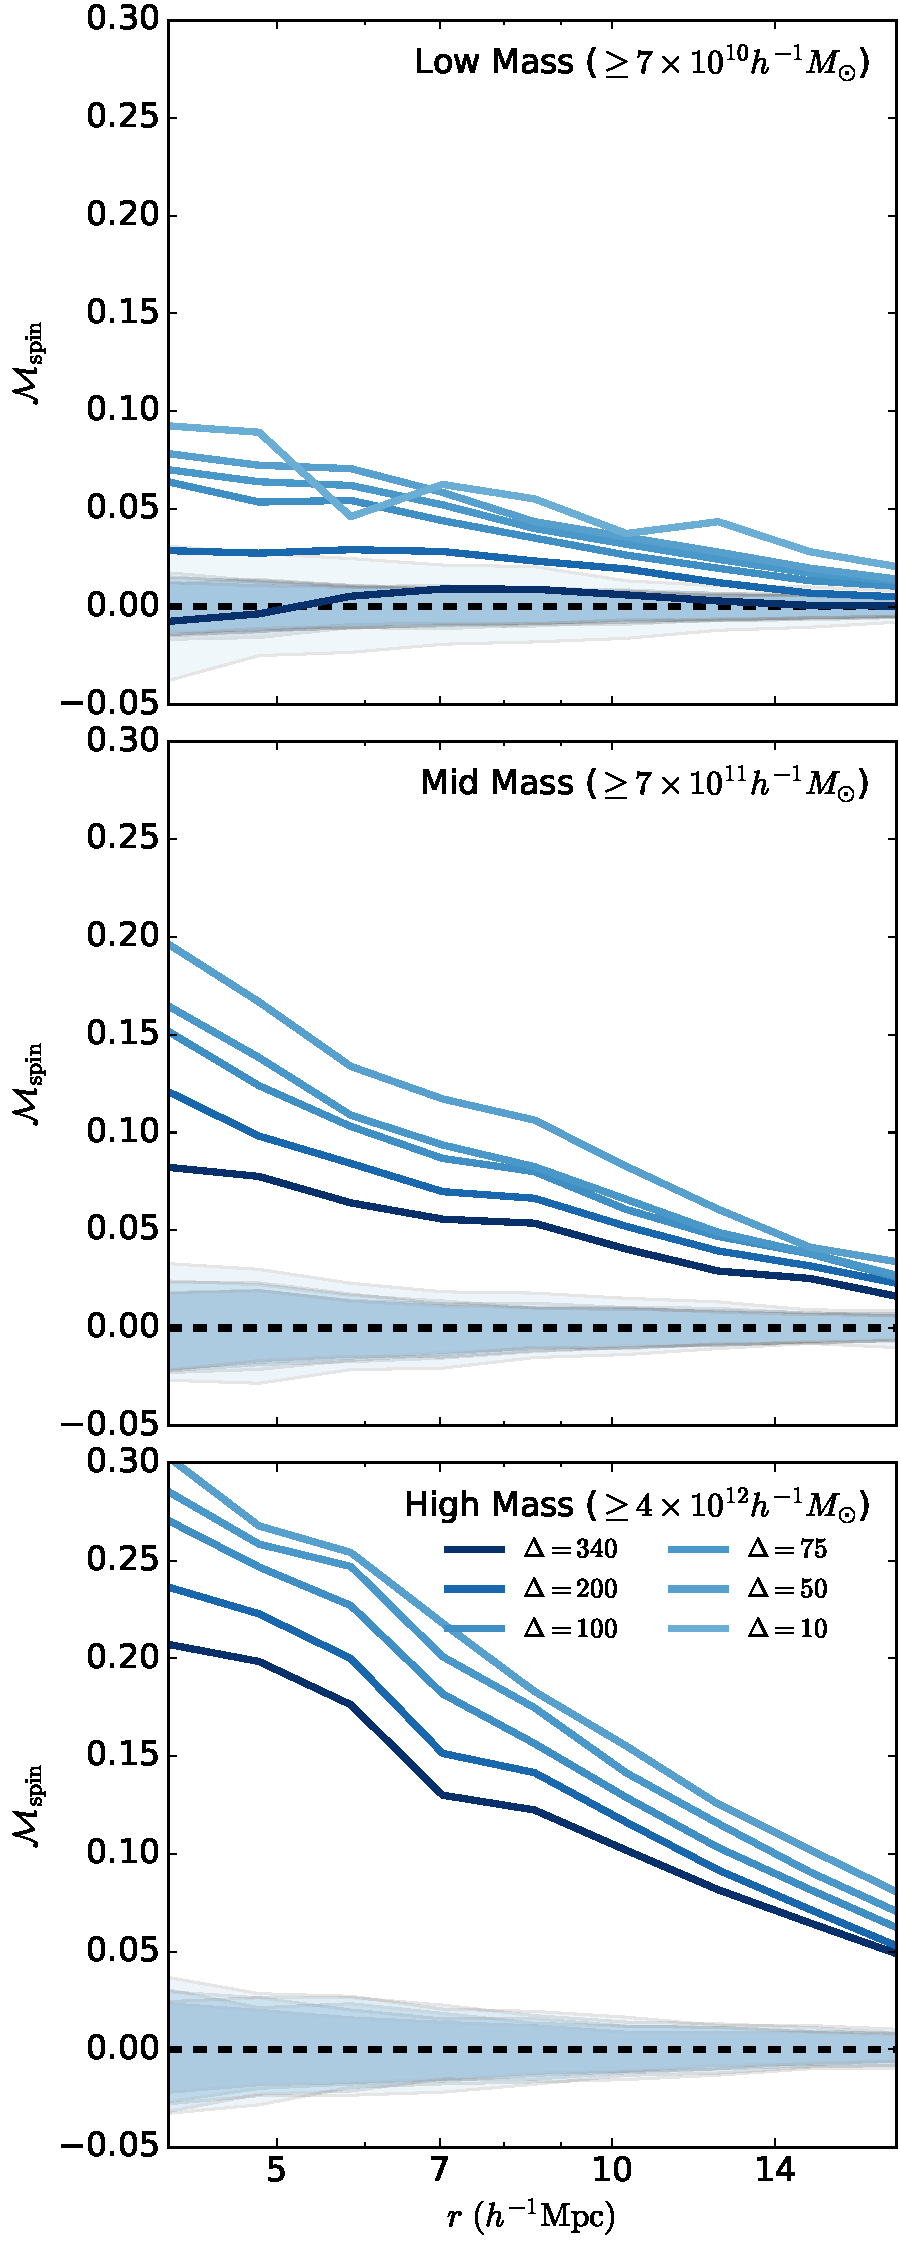
\includegraphics[width=.4\textwidth]{all_mcf_spin.pdf}
	\caption{The marked correlation function for the halo spin parameter. The solid lines plot the marked correlation function using halo spin as the mark. In each plot the line with the most 
positive value corresponds with the smallest value of overdensity parameter, 
$\Delta$, and demonstrates a smooth trend down to the largest value of 
$\Delta$. The top (middle/bottom) panel shows the results for the
\simA \ (\simB /\simC) data set utilizing the low mass (mid mass/high mass) cutoffs. Note
that the top panel is the only one where exploring the extreme regime of $\Delta = 10$ is
necessary, while the bottom panel is the only one where the exploration of $\Delta = 340$
is necessary. The shaded bands represent 2-sigma confidence regions generated by randomization of the marks.
	}
	\label{fig:cc_mcf_spin}
\end{figure}
%-------------------------------


%----------------- satellite number MCF
\begin{figure}
	\centering
	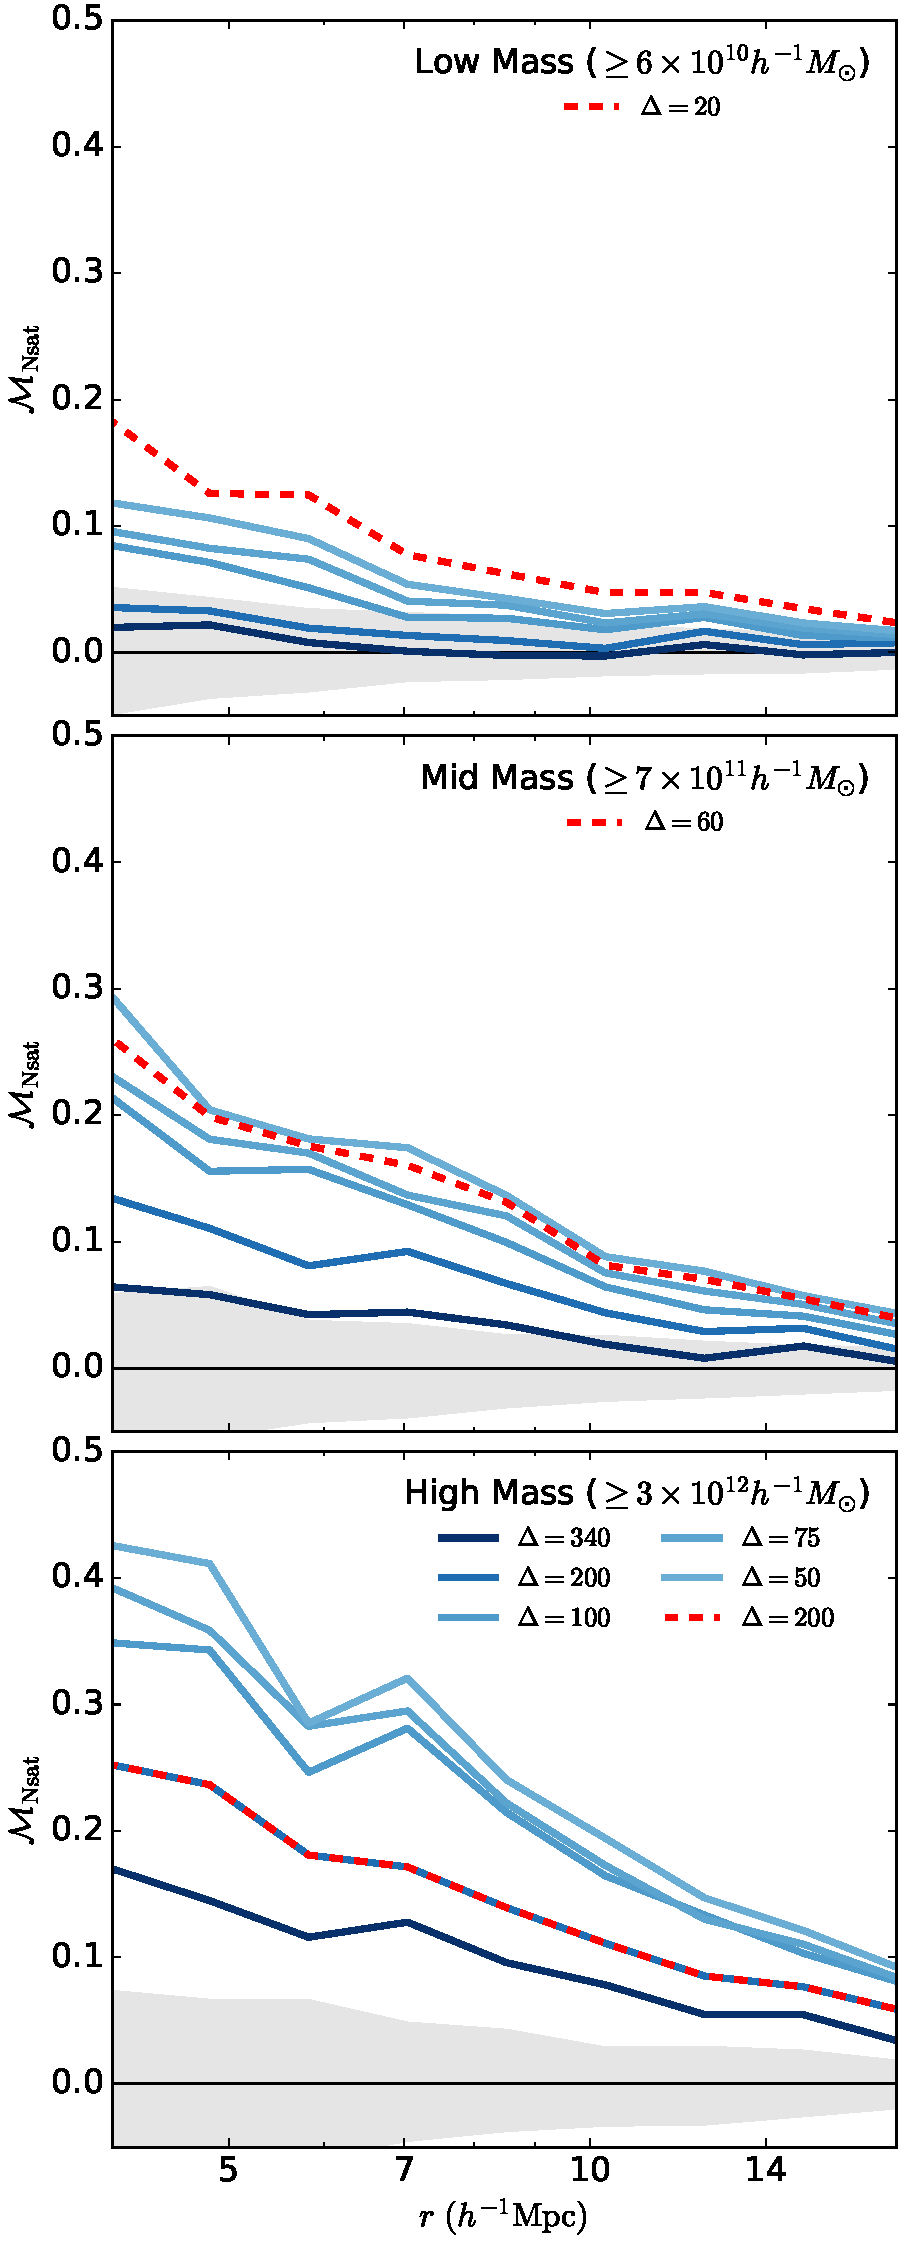
\includegraphics[width=.4\textwidth]{all_mcf_nsat.pdf}
	\caption{The marked correlation function for the satellite number parameter. The solid lines plot the marked correlation function using halo satellite number as the mark. In each plot the line with the most 
positive value corresponds with the smallest value of overdensity parameter, 
$\Delta$, and demonstrates a smooth trend down to the largest value of 
$\Delta$. The top (middle/bottom) panel shows the results for the
\simA \ (\simB /\simC) data set utilizing the low mass (mid mass/high mass) cutoffs. Note
that the top panel is the only one where exploring the extreme regime of $\Delta = 10$ is
necessary, while the bottom panel is the only one where the exploration of $\Delta = 340$
is necessary. The shaded bands represent 2-sigma confidence regions generated by randomization of the marks.}
	\label{fig:cc_mcf_nsat}
\end{figure}
%-------------------------------------------------------------------------------------------


The clustering of halos as a function of the number of satellite galaxies at fixed mass is of 
particular practical interest. Efforts to model survey data on the large-scale galaxy distribution, 
such as the halo occupation distribution (HOD) or conditional luminosity function (CLF) formalisms 
typically make the assumption that the multiplicity of satellite galaxies within a host dark matter 
halo depends solely upon halo mass. If this assumption is violated, then the phenomenological 
modeling of galaxy clustering can be more complicated than in these simplest scenarios.

Figure~\ref{fig:cc_mcf_nsat} shows clustering marked by satellite number as described in 
\S~\ref{section:methodology}. For all values of $\Delta$, halo clustering is strongly dependent 
upon satellite occupation at all masses. Interestingly, altering halo definitions as we have 
makes little difference to this dependence. In fact, defining halos to have larger radii (smaller 
$\Delta$) generally makes the environmental dependence of halo clustering more 
significant. Of course, our results pertain to satellite halos, or subhalos, rather than 
satellite galaxies, so the connection to observations and how one might 
model observed galaxy clustering is indirect, yet suggestive. 


%---------------------------------------------------------------------------------------------
\section{Discussion}
\label{section:discussion}
%---------------------------------------------------------------------------------------------

\arz{Repeating this comment here because of its importance. Look in the literature 
to see if spin-dependent halo clustering has been measured in the literature before. 
Look at http://arxiv.org/abs/1207.4476.}

We have confirmed that for conventional halo definitions 
halo clustering strength is a strong function of ``auxiliary properties" halo concentration (either measured
through a fit to the NFW profile or assigned non-parametrically as the ratio of the maximum circular velocity to
the virial velocity), halo shape, halo spin, and number of subhalos 
for host halos over a wide range of masses. These findings are consistent 
with the now significant literature on the subject subject of halo assembly bias. \citep{peacock_smith00, wechsler_etal02,
sheth_tormen04, gao_etal05, zentner_etal05, allgood_etal06, harker_etal06, wechsler_etal06, croton_etal07, dalal_etal08, mao_etal15, sunayama_etal16}
\arz{Reiterate citations here.}\asv{I THINK this covers our bases, but my lit notes might be bad.}

We have explored the efficacy of alternative halo definitions to mitigate the dependence of halo 
clustering on these ``auxiliary properties." Rather generally, we find that these alternative definitions 
do {\em not} mitigate the effects of assembly bias. In most cases, defining halos to have significantly 
larger radii (lower $\Delta$) than in conventional halo definitions had only a modest influence on 
these assembly bias effects. Moreover, to the degree that these modified halo definitions had 
any effect at all, it was often of the sense of 
making the assembly bias effect stronger, rather than weaker. 

One exception to this general conclusion is the case of halo concentration. 
Our results suggest that halo redefinition may be able to mitigate concentration 
dependent halo clustering. This is evident in Fig.~\ref{fig:cc_mcf_cnfw} and 
Fig.~\ref{fig:cc_mcf_cV}. Halo concentration is strongly correlated with halo formation 
time, so this suggests that such a redefinition may also aid in reducing assembly bias 
associated with halo formation time; however, this is a non-trivial extrapolation of our 
results and a follow-up study to assess halo formation times in alternative halo definitions 
is both interesting and warranted. 

Clearly, the halo definition that best mitigates 
concentration-dependent assembly bias must be mass dependent. Low 
values of $\Delta$ ($\Delta \sim 25$ with $R_{25} \sim 2R_{200}$) seem appropriate near for our lowest 
mass-threshold sample (with $M_{200} \ge 7 \times 10^{10} \hMsun$) whereas $\Delta \sim 200$ or slightly higher
is adequate for our highest mass threshold sample (with $M_{200} \ge 4 \times 10^{12} \hMsun$). This result is
reminiscent of much recent work on the so-called halo ``splashback radius."\citep{more_etal15} We note that while
the splashback radius methodology does seem similar in concept to our methodology, 
Fig. ~\ref{fig:splashback_compare} demonstrates that a one-to-one comparison between the two methods is difficult
at best. While both our method of halo redefinition and their determination of splashback radius seem to show a
monotonic trend in mass, we note that our work with the lowest mass halos requires a definition of halo radius
that substantially larger than the splashback radius method alone might suggest.
\arz{Here, compare our results to the splashback radius work.}

\begin{figure}
	\centering
	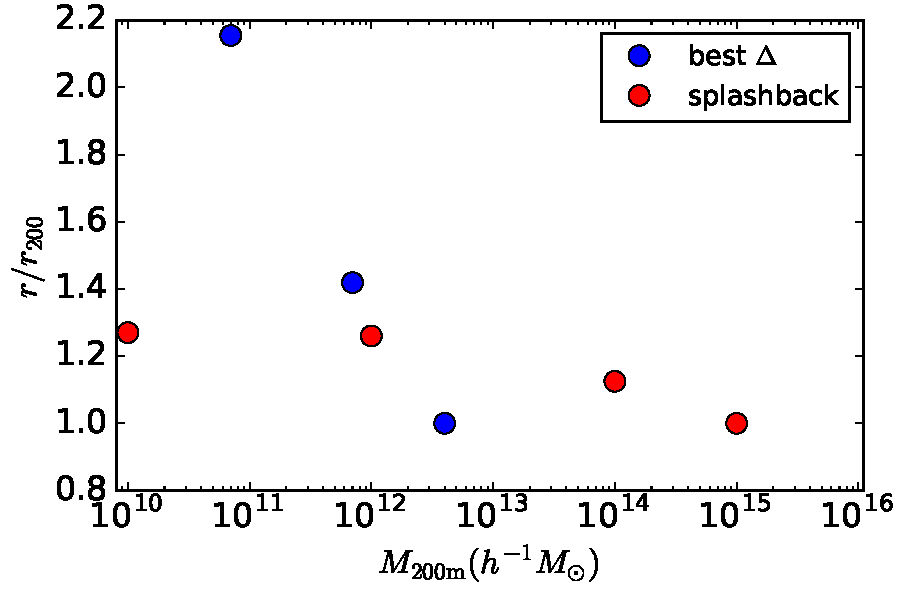
\includegraphics[width=.4\textwidth]{test_splashback.pdf}
	\caption{A comparison of the average ratio between $r_{200}$ and the splashback radius as determined by
	 \citet{more_etal15} (red circles) to the average ratio between $r_{200}$ and the halo radius determined as our
	  best fit for removal of assembly bias as discussed above (blue circles). Note that the halo mass chosen for
	  the blue points is determined by the mass cutoff in the simulation analysis, as the smallest (and most
	  numerous) halos dominate the calculation.}
	\label{fig:splashback_compare}
\end{figure}

\arz{Here is where we could use ANOTHER FIGURE! What I would like to see is a visual 
comparison of our ``best" $\Delta$ as a function of halo mass threshold compared to 
the equivalent for the splashback radius. To be clear, it is trivial to go back and forth between 
$\Delta$ and radius (since radius $\propto \Delta^{-1/3}$) so this can be represented with 
either $\Delta$ or radius. If you choose to use radius, then it should probably be normalized, 
such as $R_{\Delta}/R_{200}$ and $R_{\rm splashback}/R_{200}$ and so on. This could 
be an important figure and point to future work on this subject.}
\asv{Working on creating this plot from the splashback radius paper.}
\asv{New figure done and should be added in during the next iteration with
all new figures.}\asv{And added.}


It is useful to investigate the reasons why halo redefinitions may be helpful in the case 
of concentrations. On the positive side, it is possible that these redefinitions do define 
halos an a more practically useful way, better isolating objects that have been strongly 
altered by nonlinear evolution from the larger-scale environment. In this case, halo redefinition 
would be a step forward. However, it is also possible that the details of measuring halo 
properties using these new halo definitions introduce new sources of noise into the 
measurements. If this is the case, then the reduction in environmental effects stems 
from the fact that them measurement of the halo property 
introduces noise and is {\em less} informative about the halo itself. 
For the case of halo concentration, which is the most interesting to 
follow up, introducing noise can happen in numerous ways. For example, 
the NFW concentration $c_{\mathrm{NFW}}$ is determined by a fit to the 
NFW profile. Inferred values of $c_{\mathrm{NFW}}$ will depend upon 
the degree to which the density profiles of the halos follow the NFW 
functional form within some radius $R_{\Delta}$ that is different from 
traditional halo radii, such as $\sim R_{200}$. At large halocentric 
distances ($r \gtrsim R_{200}$) halo profiles are known to deviate 
from the NFW form. It is worth noting that the velocity-defined concentration 
$c_{\rm V}$ is a non-parametric measure of concentration and should be 
less subject to such effects. 


\arz{New figure needed here. This should be, for the L0250 simulation (my 
guess this one is most instructive, but use your judgment here), a 
comparison of the concentration-mass relation for halos defined with 
$\Delta=200$ to the concentration-mass relation for halos defined with 
$\Delta=70$ (of whatever you deem best). The figure must represent 
both the mean (or median) relation AS WELL AS the dispersion in 
this relation at fixed mass. The plot should exhibit this for both 
$c_{\mathrm{NFW}}$ and $c_{\mathrm{V}}$. Two panels may be 
necessary to make these points.}
\asv{contemplating how best to show this - currently making a running median plot, as in the masscut plots above.}
\asv{Figure is made and will be run on the new dataset and included. It
suggests that we are not significantly changing the dispersion. Numbers
added below for now.}

\begin{figure}
	\centering
	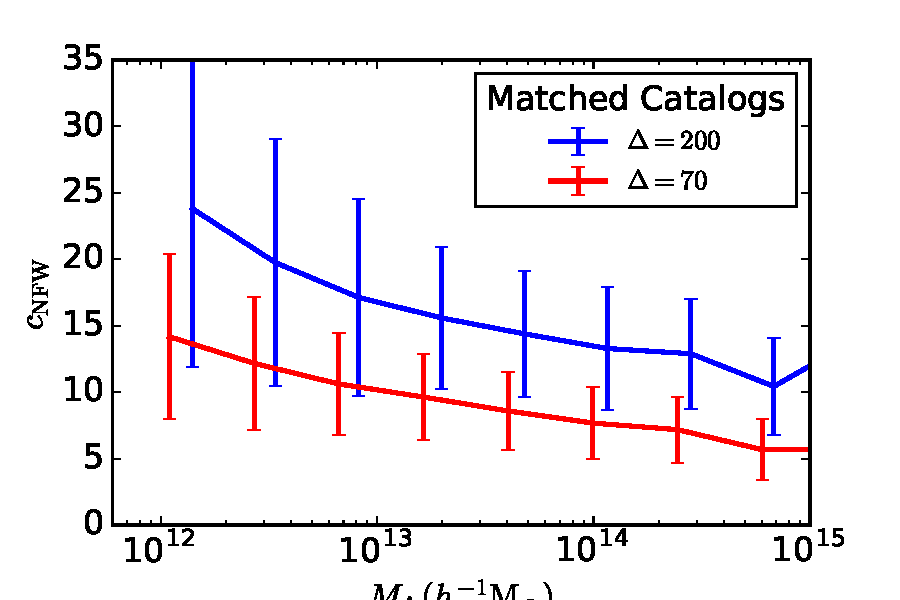
\includegraphics[width=.4\textwidth]{matched_catalog_cnfwcomp.pdf}
	\caption{A comparison of the mean value of the NFW-defined halo concentration for halos matched across both
	the $\Delta = 200$ and $\Delta = 70$ catalogs for \simB. The blue (red) line shows the mean value and scatter of
	the	mean for the $\Delta = 200$ ($\Delta = 70$) catalog. Note that there is no significant
	increase in the scatter of the mean due to the change in halo definition.}
	\label{fig:matched_cnfwcomp}
\end{figure}

As such, it is useful to examine the concentration-mass relations for halos in 
the simulations for various halo definitions. This is shown in Fig. ~\ref{fig:matched_cnfwcomp}. 
Notice that the mean dispersion of halo concentrations for a given mass
bin are not significantly changed as we move to our best fit value of
overdensity parameter, $\Delta$. This is highly suggestive of the fact
that the success of our method is not the result of larger measurement
error, but is more fundamental to the nature of relating halo definition to
our halo parameters of interest.\arz{Now you mention the interesting part about the new figure. 
This should be a discussion of how much larger/smaller the dispersion in 
concentrations gets for, say $\Delta=70$ compared to $\Delta=200$.}
\asv{The dispersion of halo concentrations is not significantly changed -
while a little smaller, it is well within the scatter of the dispersion as
well.}

We can explore in more detail the degree to which the mitigation of environmental 
effects by halo redefinition are due to introducing noise that is uncorrelated with 
environment into the measurement of halo properties when halos are defined 
in a manner distinct from the more traditional definitions. We proceed as follows. 
All host halos that are found in the halo catalogs constructed from lower values 
of $\Delta$ (for example, $\Delta ~ 70$ which is an interesting value for exploring 
concentration in the L0250 simulation) are present as host halos in the halo 
catalogs constructed with higher values of threshold density (e.g., $\Delta = 200$). 
We match each halo in the lower threshold (lower $\Delta$) simulation to 
its corresponding halo in the higher threshold catalog. We then consider 
the clustering of only those halos that we have matched across catalogs. 
We refer to these as the ``matched" halo samples between two values 
of threshold overdensity $\Delta$. 

\arz{I removed the correlation function comparison here. It is too busy to read and not necessary. 
It also opens up the whole Pandora's box of ``why choose 20\%?" I'd rather avoid that in this 
discussion. Let's just jump straight to the MCF. This will reduce the proliferation of figures as 
well.}\asv{Seems entirely reasonable. I'm starting to see \ref{sub:cfresults} as more of a proof of concept comparing to MCF results for those more
comfortable working with 2pt functions.}

\begin{figure}
	\centering
	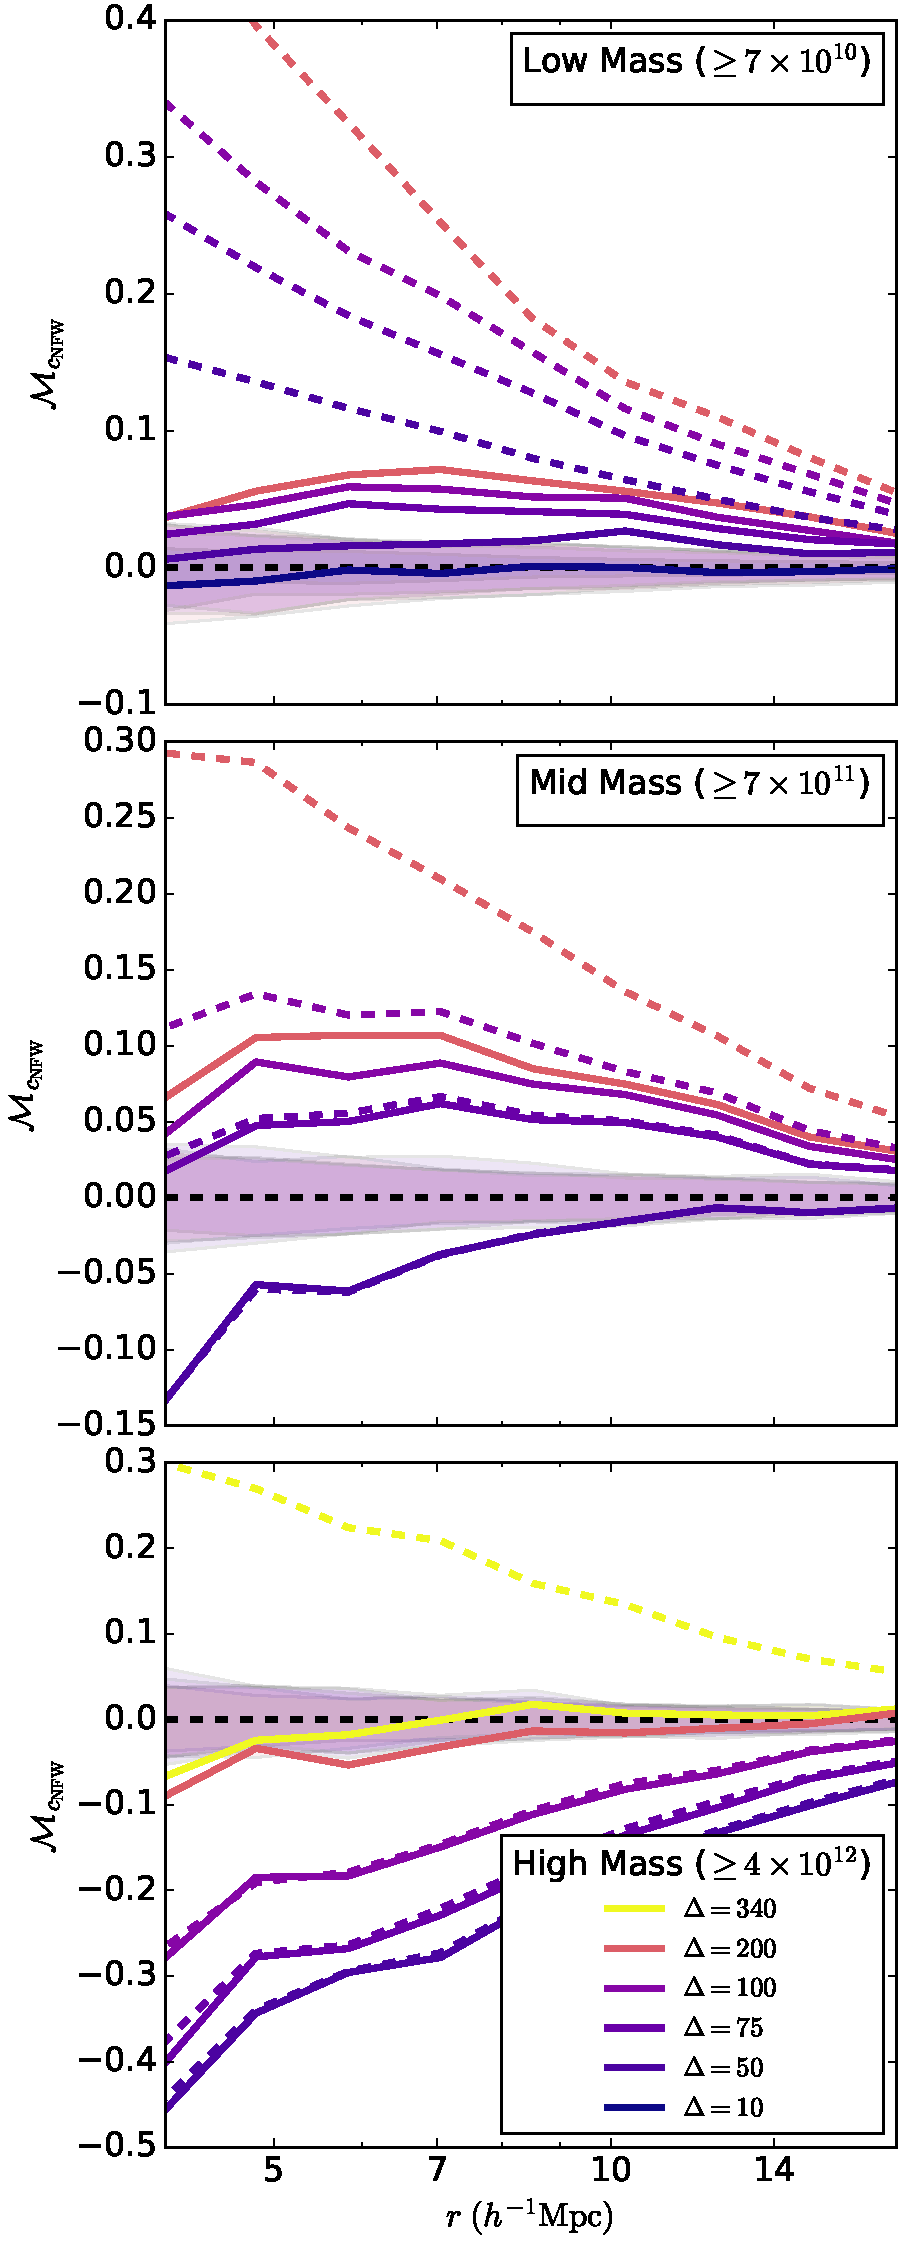
\includegraphics[width=.4\textwidth]{match_mcf_cNFW.pdf}
	\caption{The marked correlation function for the NFW-defined halo concentration parameter. The solid lines plot the marked correlation function using NFW-defined halo concentration as the mark. In each plot the line with the most 
positive value corresponds with the smallest value of overdensity parameter, 
$\Delta$, and demonstrates a smooth trend down to the largest value of 
$\Delta$. The top (middle/bottom) panel shows the results for the
\simA \ (\simB /\simC) data set utilizing the low mass (mid mass/high mass) cutoffs. Note
that the top panel is the only one where exploring the extreme regime of $\Delta = 10$ is
necessary, while the bottom panel is the only one where the exploration of $\Delta = 340$
is necessary. The shaded bands represent 2-sigma confidence regions generated by randomization of the marks. Only host halos consistent with the best-fit catalog from above are included in the analysis.}
	\label{fig:hvm_mcf_cnfw}
\end{figure}

\arz{Please check to ensure that I know what you mean by your matched samples. Your language was not 
specific enough for me to be 100\% sure. Modify as necessary.}
\asv{Looks absolutely correct to me.}
Figure~\ref{fig:hvm_mcf_cnfw} shows the same statistic as Figure~\ref{fig:cc_mcf_cnfw}, except for matched
subsamples. The matched subsamples are matched to a catalog generated for the value of $\Delta$ most likely to
remove assembly bias at large scales for the concentration marks; $\Delta=10$ for the `\simA -gen' cut, $\Delta=70$
for the `\simB -gen' cut, and $\Delta=200$ for the `\simC -gen' cut. These matched halo catalogs only differ from
the standard halo samples in that they contain only those host halos common 
to both the catalog in question and the best fit $\Delta$ catalog. The most interesting matched sample to 
examine in this case is the $\Delta=200$ sample. In this sample, all halos are defined as they would be 
defined in the $\Delta=200$ catalog, including all inferred halo properties; however, the matched catalog 
contains only those host halos that also appear in the $\Delta=70$ halo catalog. Therefore, many host 
halos have been removed from the sample because they have become subhalos in the $\Delta=70$ 
catalogs. 

From Fig.~\ref{fig:hvm_mcf_cnfw}, it is apparent that some degree of assembly bias persists in the matched 
samples. Yet, what is interesting is that a very significant fraction of the assembly bias effect has been 
removed compared to the standard $\Delta=200$ result. The halos in the matched catalogs have the 
same properties (including $c_{\mathrm{NFW}}$) as those in the standard catalogs, so that removal 
of assembly bias is {\em not} due to introducing noise or other systematics into the measurement of 
concentration. That mitigation of assembly bias is due to the halo redefinition and, in particular, 
subsuming those halos most subject to assembly bias effects as subhalos of the $\Delta=70$ 
halos. This is an interesting result suggesting that seeking optimal halo definitions may be 
one avenue to more completely separating the strongly nonlinear evolution occurring within 
halos from large-scale evolution and mitigating assembly bias. 


\begin{figure}
	\centering
	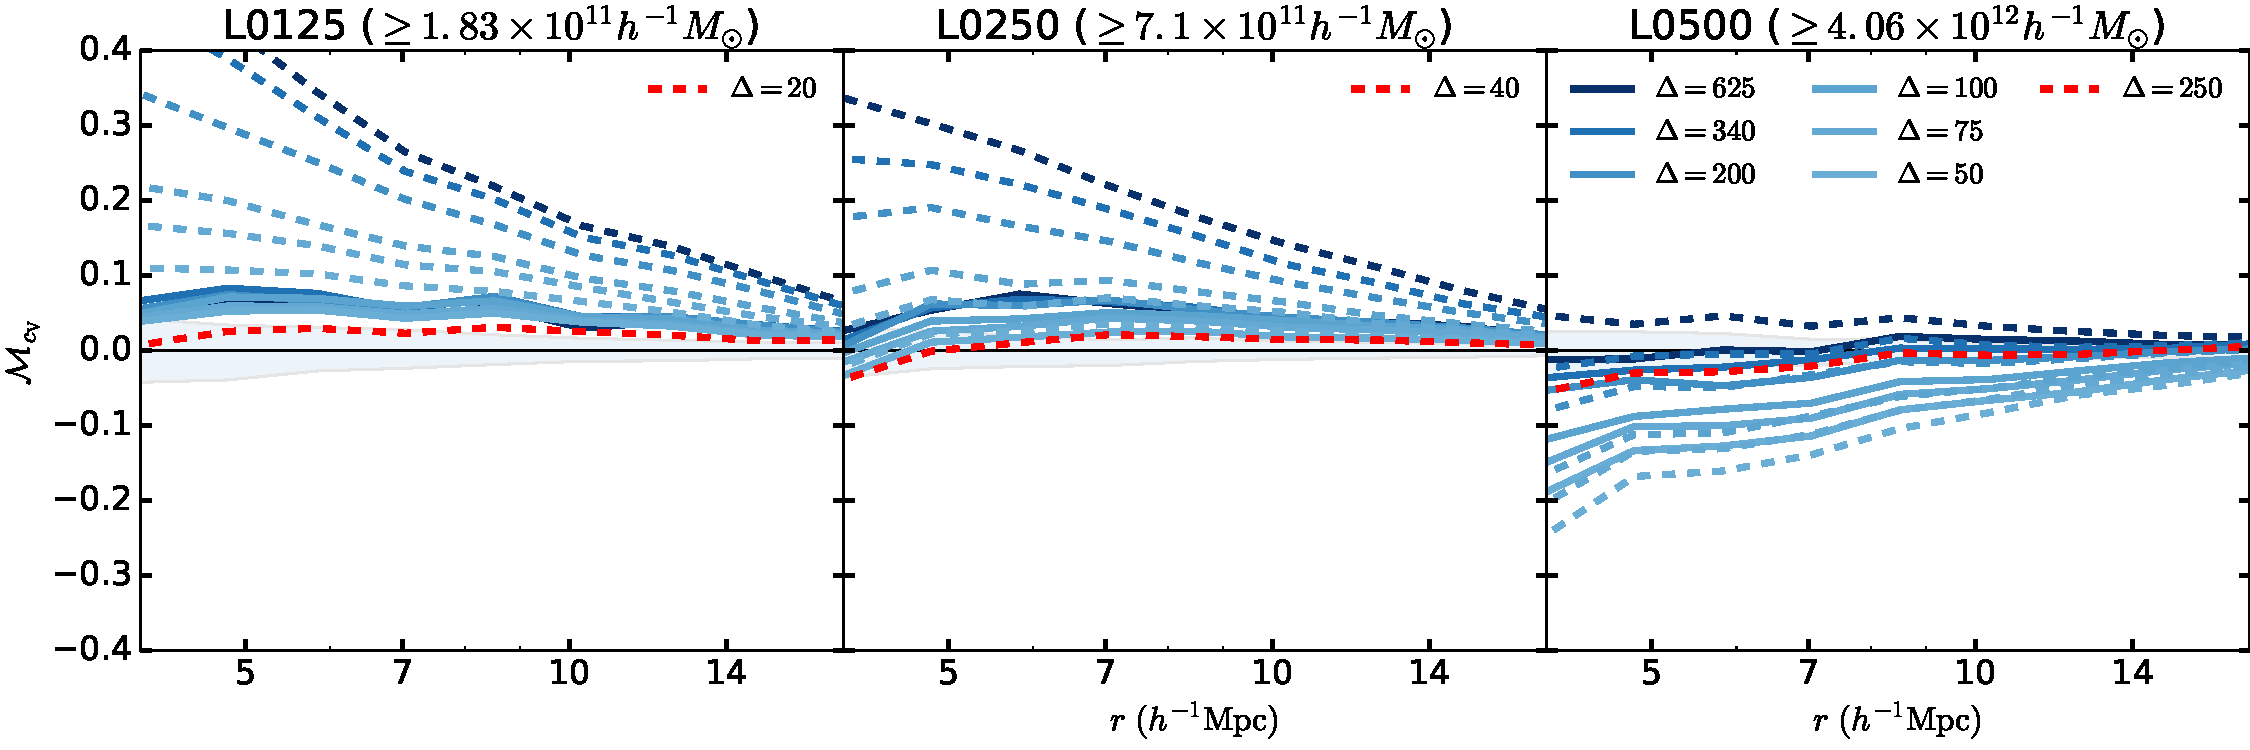
\includegraphics[width=.4\textwidth]{match_mcf_cV.pdf}
	\caption{The marked correlation function for the velocity ratio defined halo concentration parameter. The solid lines plot the marked correlation function using velocity ratio halo concentration as the mark. In each plot the line with the most 
positive value corresponds with the smallest value of overdensity parameter, 
$\Delta$, and demonstrates a smooth trend down to the largest value of 
$\Delta$. The top (middle/bottom) panel shows the results for the
\simA \ (\simB /\simC) data set utilizing the low mass (mid mass/high mass) cutoffs. Note
that the top panel is the only one where exploring the extreme regime of $\Delta = 10$ is
necessary, while the bottom panel is the only one where the exploration of $\Delta = 340$
is necessary. The shaded bands represent 2-sigma confidence regions generated by randomization of the marks. Only host halos consistent with the best-fit catalog from above are included in the analysis.}
	\label{fig:hvm_mcf_cV}
\end{figure}

\arz{Put a discussion of Fig.~\ref{fig:hvm_mcf_cV} here. It does not need to reiterate the discussion of 
Fig.~\ref{fig:hvm_mcf_cnfw}. However, it should state that we reach the same broad conclusion and that 
this is good in part because $c_{\mathrm{V}}$ is a nonparametric measure of halo concentration.}
Figure~\ref{fig:hvm_mcf_cV} follows the same exercise as above, with a comparison drawn to the Fig.~\ref{fig:cc_mcf_cV}. Notice that the same trends as Fig.~\ref{fig:hvm_mcf_cnfw} can be seen: a significant fraction of assembly bias is removed as compared to the unmatched catalog, though statistically significant assembly bias remains. Only in combination with halo redefinition do we remove assembly more completely on large scales. Note that the max circular velocity defined concentration is nonparametric by design; this helps to confirm that our result is not related to choice of halo density profile.


\arz{Would it be easy for you to plot the concentration-mass relation for only those host halos 
in the ``matched" $\Delta=200$ sample? If so, that would be potentially interesting for our 
interpretation.}\asv{In progress for above.}

\arz{This paragraph is good, but needs to be written a bit more professionally. Start with a sentence like, 
``It is interesting to explore the reasons that halo shape, spin, and satellite number are not amenable 
to having their assembly bias mitigated through simple halo redefinitions." Then move on to some specifics.}
\asv{attempted to rewrite more professionally!}

While halo shape, spin, and satellite number are not amenable to having their assembly bias mitigated through the
simple halo redefinition technique we have suggested, the underlying reasons for this behavior remains of
interest for exploration. In the case of halo shape, we suggest that the assembly bias may be driven through
interactions with large scale structure. Studies have shown a statistically significant alignment between
filaments and satellite galaxy position \citep{tempel_etal15, velliscig_etal15}\asv{need to grab paper from arxiv
2016.05.09 for this}.

Note that the mass dependence of assembly bias is implicitly explored with our suite of simulations.
The nature of the MCFs emphasizes halos just above the threshold mass; e.g. \simA~ probes the smallest mass
halos, while \simB~ probes the largest mass halos. To more explicitly explore this mass dependence, Figure~\ref{fig:biascompare}
demonstrates how bias scales as a function of both fixed halo mass and choice of overdensity $\Delta$.
There are two clear trends to be determined from this data. The first is the trend for the assembly bias with
halo concentration to be reduced as a function of halo mass. This trend helps to resolve the apparent
inconsistencies in measures of assembly bias in the literature; namely, a change in halo mass of
interest can lead to a considerably different measure of halo assembly bias - at high masses, halo assembly
bias due to NFW-defined concentration is fairly minimal. The second visible trend is that a change in halo
definition chosen has a trend of decreasing the halo bias determined. Furthermore, it should be noted that this
can lead to an anticlustering of halos of high concentration at high masses. These two discoveries seem to
suggest that halo assembly bias of NFW-defined halo concentration is a coincidence; choosing a halo size
across all halo masses as a function of an overdensity will be insufficient in creating self-similiar dark
matter halos.
\arz{Instead, add one summarizing paragraph here discussing the mass dependence of assembly bias. 
Emphasize that our findings suggest that the strength of assembly bias can be a strong function of halo 
definition and that this may already be making it difficult to compare the results of various different research 
groups using different halo definitions.}

\begin{figure}
	\centering
	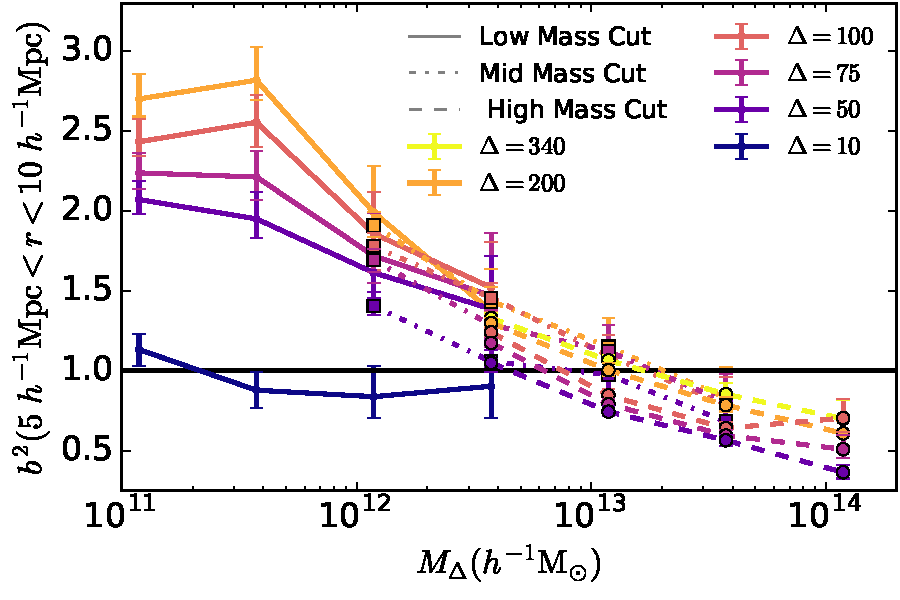
\includegraphics[width=.4\textwidth]{biasplot.pdf}
	\caption{The bias with respect to NFW-defined halo concentration against halo mass measured at the halo
	radius. The displayed lines descend from highest values of overdensity parameter $\Delta$ in that mass
	range to the lowest value. The low mass range (dotted lines) covers from $\Delta=200$ to $\Delta=10$, 
	the mid mass range (dashed lines) covers	from $\Delta=200$ to $\Delta=50$, and the 
	high mass range (solid lines) covers from $\Delta=340$ to $Delta=50$. The
	error bars show where 68\% of bias measurements lie within sampling noise. The solid black line
	shows where there is no assembly bias driven by NFW-defined halo concentration.}
	\label{fig:biascompare}
\end{figure}


%----------------------
\section[]{Conclusions}
\label{section:conclusions}
%----------------------

\arz{After dealing with the comments above, let's come back to rewriting the conclusions section.}
We have looked at how to use CFs and MCFs in order to analyze the environmental effects upon the properties of the halo. We have suggested a method of removing the mass dependence that is not subject to the small number statistics at large halo masses. Taking our various tests, we then apply a change to the threshold density $\Delta$ in an attempt to remove the effect that environment has upon these properties. We come to the following conclusions from our simulation data.

\begin{itemize}
	\item Our halo redefinition method does not cause any substantial breakdown in the ROCKSTAR halo finding
algorithm, though this may not be the case for every halo finding methodology. This is something that should be
considered prior to utilization of this method, unless working directly from particle data. As our initial halo
sizes and locations are determined through spherical overdensities, it cannot be assumed that starting from a FoF
grouping and then determining values through particle data directly will produce identical results. Similarly,
different cosmologies may remove environmental effects at different scales.

	\item When looking at the two-point correlation function, there appears to be a ``sweet spot'' that appears
to remove environmental effects the most efficiently. Going beyond that seems to reintroduce environmental
effects, possibly as an extreme side effect of halo exclusion.

	\item For our marked correlation functions we see that both proxies of concentration that we use as marks
show significant removal of environmental effects at large scales for similar values of the overdensity parameter
$\Delta$. In cases where one is only interested in the concentration of dark matter halos and large scales (or
correspondingly small values of k), this method will allow you to compensate for bias that environment could
introduce to calculations dependent upon the halo model. This may prove valuable for calculations such as that of
the shear power spectrum calculated through weak lensing.

	\item The environmental effects on the shape of the host halo and the satellite number of the host halo
cannot be removed regardless of the chosen redefinition of $\Delta$. We propose that this may be intrinsically
tied to the nature of the filaments, whose effects cannot be removed by a simple redefinition of the halo radius.

	\item This method is definitively related to the mass of the halos that are being observed. Furthermore, it
appears that the majority of the reduction in assembly bias is tied to the exclusion of halos from the catalog as
a result of being subsumed into larger halos. This information does not seem to be contradictory; it can be
intuitively understood that the region about the most massive halos will be different than the region around the
least massive halos, leading to a different frequency at which halos are being excluded. It does however warrant
that careful consideration be given to the sample of halos that are of interest.

	\item The selection of halo size is intrinsically related to the assembly bias and varies across scales. This
might help to resolve contradictory results in the search for halo assembly bias in the literature.
\end{itemize}

This methodology, while certainly not perfect in accounting for assembly bias, may be of significance when
applied to galaxy formation models and give insight into seemingly conflicting results. Provided that the
properties of interest in a given model behave well under our redefinition, it will allow us to create better
mock galaxy catalogs without resorting to more complicated models requiring halo formation histories - giving us
another powerful tool to test observation against.

There remain possible uncertainties to study in the future. One possible area of follow-up is the matter of
simulation cosmology, which is not explored in this text. It is possible that the choice of cosmology may change
observed assembly bias as a function of the halo masses, something that our methodology should be capable of
observing. Furthermore, we can determine if the choice of halo size that best reduces assembly bias is a function
of the chosen cosmology. This may be of interest in attempting to determine signatures of assembly bias in
observational samples in the future.

\section*{Acknowledgments}

We are grateful to many people. Our calculations are carried out utilizing the
{\tt numpy} \citep{numpy}, {\tt astropy} \citep{astropy}, {\tt matplotlib} 
\citep{matplotlib}, and {\tt halotools} \citep{halotools} packages in Python.

%%\bibliographystyle{plainnat}
\bibliography{master}

\section*{Appendix}
\label{section:appendix_massres}

One natural question that might arise in the analysis of this work is the nature of the resulting assembly bias
trends. Our focus in the main sections of this paper is on the nature of the assembly bias changing as a function
of the mass cut chosen. Our conclusions include the fact that there is a strong mass dependence on halo assembly
bias that must be accounted for separately depending on the halos of interest in a study. However, while the
existence of this trend is clear within our analysis, the determination that this is solely due to the masses of
the halos included in our calculation is less clear upon closer inspection. One possibility that might be
particularly concerning is the potential that the different simulations have created halos that have
fundamentally different clustering and this is leading to the result that we are interpreting as a mass
dependence on assembly bias. Thankfully, though our statistics become less meaningful to carry out this
calculation, we can carry out a comparison using the same mass cut across two of our simulations, knowing that
these will only contain well resolved halos.

While not addressed directly, Figure~\ref{fig:hvl_cfcompare} through Figure~\ref{fig:hvl_mcf_nsat} contain a
demonstration of the result that we are seeking in the left column of panels. The lower left panels show various
marks of interest for \simB \ using the ``mid mass'' cut on the data set. In comparison, the upper left panel
contains the same marks of interest for the \simA \ using the same mass cut. In the latter, there are fewer halos
in this mass cut range, as a result of the smaller simulation box size. However, we note that despite the
additional noise in the data set, the behavior of the assembly bias measurement is nearly identical within
tolerances accounting for differences between simulations and noise. This motivates our conclusion that the
driver behind the behavior is the mass cut of the data sets rather than the resolution of the simulation.

\label{lastpage}

\end{document}
